\documentclass[a4paper,onesided,12pt]{report}
\usepackage{styles/fbe_tez}
\usepackage[utf8x]{inputenc}
\renewcommand{\labelenumi}{(\roman{enumi})}
\usepackage{amsmath, amsthm, amssymb}
\usepackage[bottom]{footmisc}
\usepackage{cite}
\usepackage{graphicx}
\usepackage{longtable}
\graphicspath{{figures/}}

\usepackage{multirow}
\usepackage{subfig}
\usepackage{algorithm}
\usepackage{algorithmic}
\usepackage{lipsum}

\newtheorem{thm}{Theorem}[chapter]
\newtheorem{prop}[thm]{Proposition}
\newtheorem{lem}[thm]{Lemma}
\newtheorem{cor}[thm]{Corollary}
% COVER PAGE
\title{HIERARCHICAL MIXTURES OF GENERATORS}
\turkcebaslik{ÜRETİCİLERİN HİYERARŞİK KARIŞIMLARI}
\degree{B.S., Computer Engineering, Boğaziçi University, 2017}
\author{Alper Ahmetoğlu}
\program{Computer Engineering}
\subyear{2019}

% APPROVED BY PAGE
\supervisor{Prof. Dr. Tunga Güngör}
\examineri{Prof. Dr. Ethem Alpaydın}
\examinerii{Prof. Dr. X}
\dateofapproval{DD.MM.YYYY}

\begin{document}

\pagenumbering{roman}
\makemstitle % M.S. thesis
\makeapprovalpage
\begin{acknowledgements}
Empty for now.
\end{acknowledgements}
\begin{abstract}
Generative adversarial networks are used successfully to model complex data distributions. One variant trains multiple generators each one responsible from one local mode of the data distribution. In this work, we review such approaches and propose a hierarchical mixture of generators, learning a hierarchical division in the tree structure as well as the local generators in the leaves. Since these experts are combined softly, the whole model is continuous and can be trained using gradient-based optimization. Our experiments on five image data sets, namely, MNIST, FashionMNIST, CelebA, UTZap50K and Oxford Flowers, show that our proposed model is as successful as the fully connected neural network; the learned hierarchical structure also allows for knowledge extraction.
\end{abstract}
\begin{ozet}
Generative adversarial networks are used successfully to model complex data distributions. One variant trains multiple generators each one responsible from one local mode of the data distribution. In this work, we review such approaches and propose a hierarchical mixture of generators, learning a hierarchical division in the tree structure as well as the local generators in the leaves. Since these experts are combined softly, the whole model is continuous and can be trained using gradient-based optimization. Our experiments on four image data sets, namely, MNIST, FashionMNIST, CelebA, UTZap50K and Oxford Flowers, show that our proposed model is as successful as the fully connected neural network; the learned hierarchical structure also allows for knowledge extraction.
\end{ozet}
\tableofcontents
\listoffigures
\listoftables
\begin{symbols}
% The title will be typeset as "LIST OF SYMBOLS".
%
% Use a separate \sym command for each symbols definition.
% First Latin symbols in alphabetical order

\sym{$a_{ij}$}{Description of $a_{ij}$}
\sym{$\mathbf{A}$}{State transition matrix of a hidden Markov model}
% Then Greek symbols in alphabetical order
\sym{}{}
\sym{$\alpha$}{Blending parameter \textit{or} scale}
\sym{$\beta_t(i)$}{Backward variable}
\sym{$\Theta$}{Parameter set}

\end{symbols}

\begin{abbreviations}
 % Abbreviations in alphabetical order
\sym{2D}{Two Dimensional}
\sym{3D}{Three Dimensional}
\sym{AAM}{Active Appearance Model}
\sym{ASM}{Active Shape Model}
\end{abbreviations}


\chapter{INTRODUCTION}
\label{chapter:intro}
\pagenumbering{arabic}

One of the main problems in machine learning is how to learn to predict the outcome of an event $y$ that is dependent on another event $x$. These events, $x$ and $y$, can be thought as random variables with probability distributions $p(x)$ and $p(y)$ respectively. Learning corresponds to finding the appropriate mapping $f$, that satisfies $f(x) = y$. In general, we do not explicitly know the probability distributions of these events. Rather, we are given a set of data points $X=\{x^{(i)}\}_{i=1}^{N}\thicksim p(x)$ with their respective targets $Y=\{y^{(i)}\}_{i=1}^{N}\thicksim p(y)$. We construct a function $f(x; \theta)=\hat{y}$. Every function has a set of parameters that defines the function itself. Here, $\theta$ is the set of parameters of the function. Based on our data set $X$, and corresponding targets $Y$, we tweak the parameters of the function so that $\sum_i L(f(x^{(i)}; \theta), y^{(i)})$ is minimized for a function $L$ that measures the difference between two values. From this point, the problem becomes an optimization problem. In most cases, we use gradient-based optimization techniques due to its cheap computational demand. When we use gradient-based techniques, the curvature of the function that we optimize with respect to its parameters are important. Therefore, we tend to choose $L$ to be a convex function due to a set of desired convergence properties.

In the above setting, we are concerned with the statistical regularities between $X$ and $Y$. The learned mapping $f^{*}(x)$ maps the $x$-space to the $y$-space. An alternative interpretation is that we partition the $x$-space into regions with respect to outcomes of $y$. We can think of this process as finding discriminative borders in $p(x)$ to predict the outcome of $y$. One can see that these borders are totally dependent on $y$. If there happens to be only one outcome of event $y$, then the $x$-space has no borders and there is only one color (there is only one region). On the other extreme, if each data point $x^{(i)}$ corresponds to a different target $y^{(i)}$, then each point will have a different color in the $x$-space and there will be lots of borders. Trying to learn a mapping from $x$-space to some target~$y$-space is called \emph{supervised learning}. This is supervised because we specify a target for each data point.

\begin{figure}[htbp]
\begin{center}
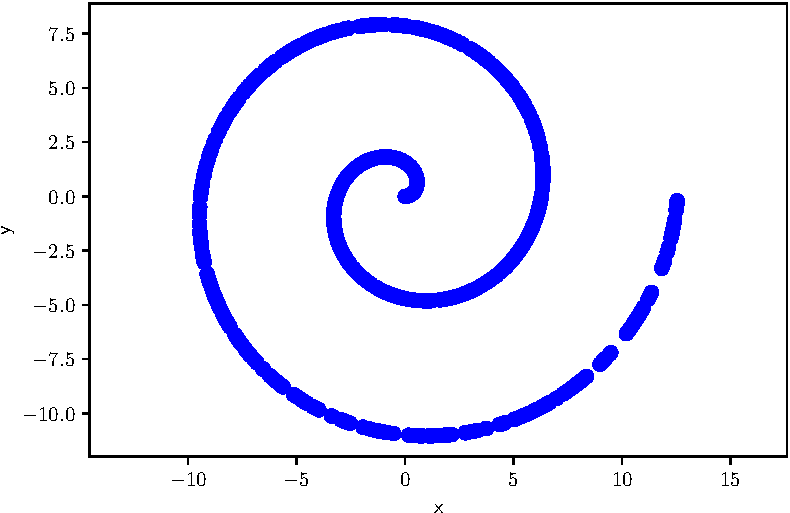
\includegraphics[width=0.6\columnwidth]{euc.pdf}
\end{center}
\caption{A spiral data set. The data is one-dimensional, if we know $x=r*cos(r)$, $y=r*sin(r)$.}
\vskip\baselineskip % Leave a vertical skip below the figure
\label{fig:spiral}
\end{figure}

Another important research direction in machine learning is \emph{unsupervised learning}. Here, we are not given a set of pre-defined targets. So we do not know the outcome of $y$ that is dependent on the given input $x$. We do not even know if there is any $y$. The aim is to model the probability distribution of $x$, to see what normally happens. Therefore the aim is to find statistical regularities within the $x$-space. However, without any supervision, it is not quite clear what is a statistical regularity. For example in Figure \ref{fig:spiral}, if we use Cartesian coordinates, we probably fail, or rather find poor estimates. If we know the transformation to polar coordinates, then we can model the distribution better by first transforming Cartesian coordinates to polar coordinates. Therefore, the transformation $\phi(x)$ is the golden nugget.

The same argument is also true for supervised learning. However, we have the information that can direct us to find appropriate transformations: targets. Previously, people searched for better transformations to increase model performance. \emph{Deep learning} approach tries to solve the problem by also learning transformations. That is, we train a multi-layer perceptron (MLP), also called artificial neural network (ANN), to estimate $p(y|x)$. The idea is to learn basic transformations at earlier layers and using them to construct higher level, more abstract transformations \cite{bengio2009learning}. When we learn abstract transformations from the data, we end up with models that have better \emph{generalization}, that is the performance on unseen data.

Apart from supervised and unsupervised learning, there also another dichotomy which we should mention: generative models and discriminative models. Discriminative models try to model the probability distribution $p(y|x)$. These are mostly used for classification tasks. On the other hand, generative models try to model $p(x, y)$. With a generative model, one can do several things: detect the probability of a new data, generate new data, and also classify data. We can use generative models as discriminative ones since we can find $p(y|x)$:
\begin{equation}
p(y|x) = \frac{p(x, y)}{\sum_{y'} p(x, y')}
\end{equation}

Deep neural networks (DNNs) achieved great success on real-world problems that requires generalization such as object recognition \cite{krizhevsky2012imagenet}, speech recognition \cite{hinton2012deep} and statistical machine translation \cite{sutskever2014sequence}. These models are discriminative models and trained in a supervised fashion. The success of \emph{deep learning} did not translate to generative models until the proposal of \emph{generative adversarial networks} (GANs) \cite{goodfellow2014generative}. This was partly because we did not know a clear objective as we did in discriminative modeling. How do we learn transformations that are good for modeling $p(x)$? How do we quantify the goodness of a transformation? At this moment, there is still no consensus on the answers of these questions.

GANs seem to be a promising way to train DNNs for generative modeling. In this thesis, we propose to use hierarchical mixture of generators as the generative part of GAN. This lets us interpret the learned representation. The rest of this work is organized as follows. Chapter \ref{chapter:gan} reviews the prerequisite knowledge about GANs. In Chapter \ref{chapter:multiple_gan}, we discuss works that also use multiple generators. We explain our proposed model in detail in Chapter \ref{chapter:mixture_gan}. Our experimental results are given in \ref{chapter:exps}. We make a conclusion and discuss future work in Chapter \ref{chapter:conc}.

\chapter{GENERATIVE ADVERSARIAL NETWORKS}
\label{chapter:gan}

\section{Introduction}
\label{sec:gan:intro}

The generative adversarial network (GAN) \cite{goodfellow2014generative} has been proposed to learn a generative model to model a data distribution, $p(x)$. GAN is composed of two learners, a generator network $G$ and a discriminator network $D$. $G(z;\theta)$ learns to map $z$ sampled from an arbitrary distribution $p(z)$ to the target distribution $p(x)$. It is a trained model, generally a deep neural network, parameterized by $\theta$. The discriminator $D(x;\phi)$, another neural network with weights $\phi$, is trained to assign low scores to ``fake'' samples generated by $G(z;\theta)$ and high scores to samples from true $p(x)$ given in the training set. We do not show any true samples to $G$, instead train it to generate samples that will get high score from $D$. This is achieved with the following objective:
\begin{equation}
\label{eq:gan}
\underset{G}{\text{min}} \quad \underset{D}{\text{max}} \quad \mathbb{E}_{x \sim p(x)} [ \log{D(x;\phi)} ] + 
\mathbb{E}_{z \sim p(z)} [ \log{(1-D(G(z;\theta);\phi))} ]
\end{equation} 

We optimize Equation \ref{eq:gan} by alternating between optimizing $D$ and $G$ with stochastic gradient descent (SGD) (Figure \ref{fig:gan}). In the original paper  \cite{goodfellow2014generative}, it is shown that if $D$ and $G$ have enough capacity, this optimization minimizes the Jensen-Shannon divergence (JSD) between $p_{\text{true}}$ and $p_{\text{fake}}$, and therefore will converge to a point where $G$ exactly generates the target distribution $p(x)$. Though it should be noted that we use a parametric family of functions defined by neural networks. This might limit our functions' capacity and break the convergence guarantee. 
%
\begin{figure}[htbp]
\begin{center}
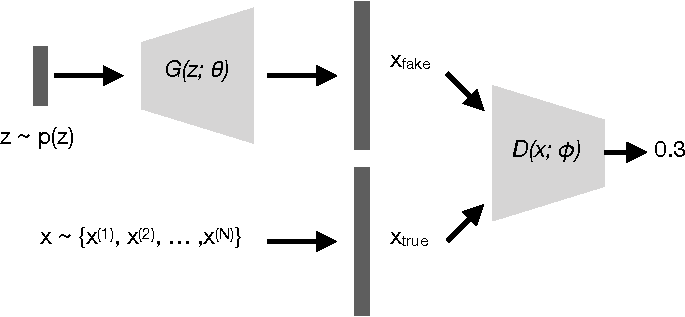
\includegraphics[width=0.75\textwidth]{gan.pdf}
\end{center}
\caption{GAN framework.}
\vskip\baselineskip
\label{fig:gan}
\end{figure}

If training converges, $G$ can generate new data simply by sampling an input point $z$, and outputting $G(z)$. On the other hand, $D$ can be used as a feature extractor for downstream tasks since it learns a good representation of $p(x)$ due to adversarial training.

\section{Problems Related with GANs}
\label{sec:problems}

GANs are used successfully especially in image generation. A well-trained GAN can generate images that are almost indistinguishable by humans \cite{karras2017progressive,brock2018large,karras2019style}. Yet, there remain two main difficulties regarding the training: The first problem of mode collapse means that $G$ learns to generate some parts of $p(x)$ but not all; there are ways of being $x$ that cannot be generated for any $G(z)$. This is depicted in Figure \ref{fig:modecollapse}. The second problem is of vanishing gradients. In order to optimize Equation \ref{eq:gan} for $G$, we should find gradients with respect to $\theta$. However $\nabla_{\theta} \log(1-D(G(z)))$ becomes zero in regions where $D$ is perfectly able to discriminate $p_{\text{true}}$ and $p_{\text{fake}}$. To remedy this, it is suggested to use a proxy loss, also known as non-saturating loss \cite{fedus2017many}: $-\log D(G(z))$. This loss provides better gradients even when $D$ is optimal. However, Arjovsky and Bottou \cite{arjovsky2017towards} showed that this loss no longer minimizes the JSD, but rather $KL(p_{\text{fake}} || p_{\text{true}}) - 2 JSD(p_{\text{fake}} || p_{\text{true}})$, where $KL$ is the Kullback-Leibler divergence. Moreover, they show that when $D$ gets better, gradients of $G$ increases with an increasing variance. They concluded that this increasing variance might be the cause of the notorious instability of GANs.

\begin{figure}[htbp]
\begin{center}
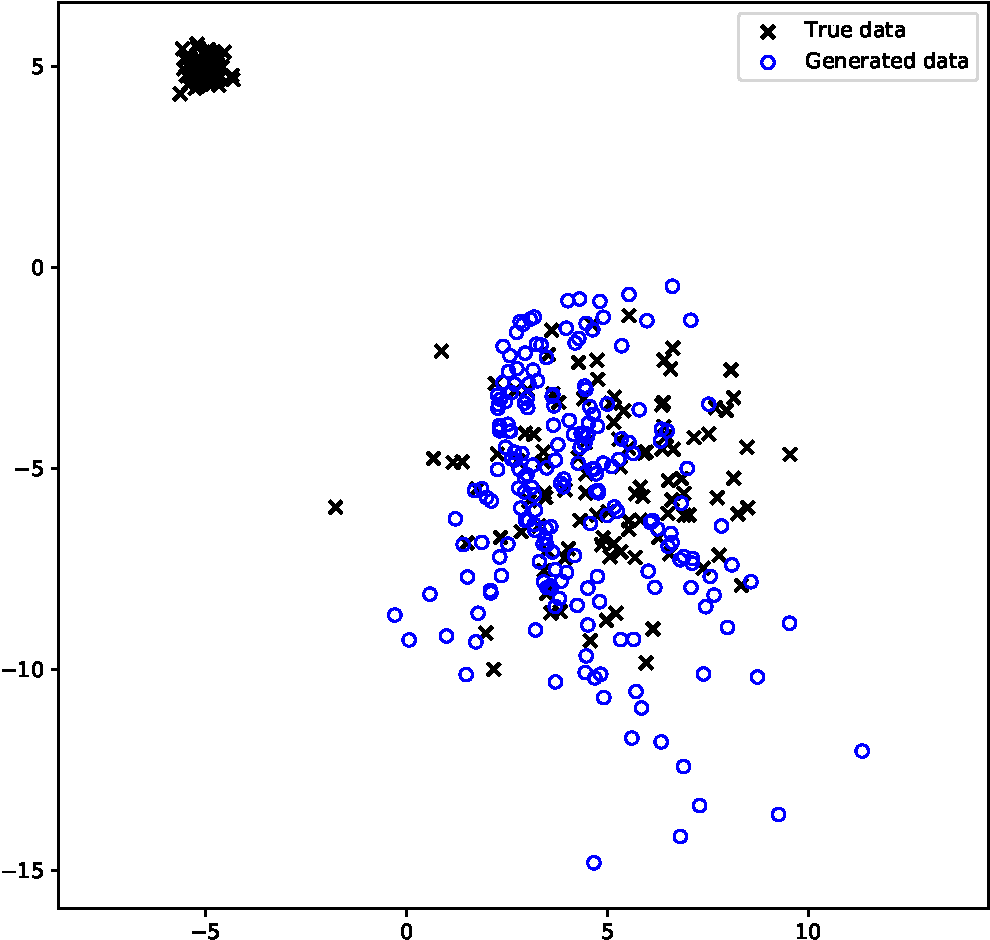
\includegraphics[width=0.5\textwidth]{modecollapse.pdf}
\end{center}
\caption{An example of a mode collapse.}
\vskip\baselineskip
\label{fig:modecollapse}
\end{figure}

Recent works mainly focus on these two problems. To solve problems related to training people proposed different GAN objectives \cite{arjovsky2017wasserstein,chen2016infogan,mao2017least,qi2017loss}, regularization methods \cite{gulrajani2017improved,miyato2018spectral,radford2015unsupervised}, architectures \cite{brock2018large,donahue2016adversarial,dumoulin2016adversarially,karras2017progressive,karras2019style,radford2015unsupervised,zhang2018self} and several other tricks mentioned in these papers. A good review of these works can be found in \cite{creswell2018generative,hong2019generative,kurach2018gan}.

\section{Variants of GAN}
\label{sec:variants}


\section{Wasserstein GAN}
\label{sec:wgan}
In \cite{arjovsky2017towards}, authors show the shortcomings of the original GAN loss (Fedus \textit{et al.} \cite{fedus2017many} call this minimax loss and we will use this notation), including the non-saturating version. If $D$ becomes optimal discriminator, then the gradients of $G$ vanish for the minimax loss. On the other hand, the non-saturating loss makes gradients unstable. One can think of training $D$ less, not until optimality, however there is no such principled way to control the optimality in GAN framework. In a follow-up work \cite{arjovsky2017wasserstein}, their motivation is to build a new distance measure that has good convergence properties even when the discriminator is optimal. They propose minimizing Earth-Mover (EM) distance, also known as 1st Wasserstein distance. The advantage is that Wasserstein distance is a convex function even when two distributions' supports do not intersect. It is defined as follows:
\begin{equation}
W_1(p_t, p_f) = \inf \quad \mathbb{E}_{(x,y) \sim (p_t, p_f)} [ \| x-y \| ]
\label{eq:emd}
\end{equation}
However, this formulation is known to be intractable. From the optimal transport view, this formulation tells us the distance is the minimum one out of all transportation plans. Instead, we use the Kantorovich-Rubinstein duality as in \cite{arjovsky2017wasserstein}:
\begin{equation}
W_1(p_t, p_f) = \underset{\|f\|_L \leq 1}{\sup} \mathbb{E}_{x\sim p_t} [f(x)] - \mathbb{E}_{x \sim p_f} [f(x)]
\label{eq:wd}
\end{equation}
where $\|f\|_L \leq 1$ implies 1-Lipschitz functions. Equation \ref{eq:wd} tells us that in order to find $W_1$ distance, we should find such $f$ that will maximize the difference. If there is no Lipschitz constraint, then we can find functions that will maximize the difference indefinitely. Lipschitz constraint ensures that we are searching the function in a bounded region.

Now, to find Wasserstein distance between two distributions, we can simply create a random neural network $f$ and maximize Equation \ref{eq:wd} with SGD. The function $f$ can be thought as a ``critic'' instead of discriminator since the output of the critic tells the generator how far it is from the true distribution. Then, for the generator, we minimize the Wasserstein distance since we know that doing so will bring two distributions closer. This formulation is called Wasserstein GAN (WGAN) \cite{arjovsky2017wasserstein}.  Differences between WGAN and GAN are:
\begin{itemize}
	\item The discriminator outputs a real value, instead of a probability.
	\item The discriminator is constrained to be 1-Lipschitz.
	\item The discriminator should be trained till optimality as opposed to GANs since better discriminator implies better $W_1$ distance, and therefore better gradients to $G$.
\end{itemize}

To enforce Lipschitz constrained, Arjovsky \textit{et al.} \cite{arjovsky2017wasserstein} suggested clipping weights of the critic function. They also warned that this is not a good way enforcing Lipschitz. A follow-up work \cite{gulrajani2017improved} introduced a more principled way by applying gradient penalty to the critic.

WGANs show better convergence properties both in theory and in practice when compared with the original GANs. For this reason, we use WGAN formulation with the gradient penalty \cite{gulrajani2017improved} in our experiments.

\section{Evaluation Metrics}
\label{sec:evaluation}

Another problem is of evaluating GANs. Unlike Bayesian generative models where we can evaluate the quality of a model with marginal likelihood (or with evidence lower bounds), there is no proper way of evaluating GAN models. At the moment, people seem to agree on Inception score (IS) \cite{salimans2016improved} and Fr\'echet Inception distance (FID) \cite{heusel2017gans} since most of papers include these scores. These two scores use Inception v3 network \cite{szegedy2016rethinking} that is pre-trained on ImageNet \cite{deng2009imagenet}.

\subsection{Inception Score}
\label{subsec:is}
In IS, the conditional class distribution $p(y|x)$ is compared with the marginal class distribution $\int_x p(y|x) p(x)$. Here, probabilities are provided from Inception network. The idea is the entropy of $p(y|x)$ should be low if $x$ contains real-looking images since we believe Inception v3 is a good image classifier. On the other hand, the entropy of $\int_x p(y | x) p(x)$ should be high if the model outputs different images, therefore different probabilities. The overall formulation is:
\begin{equation}
\label{eq:is}
\text{IS}=\exp (\mathbb{E}_{x \sim p_f} KL (p(y|x) || p(y))) 
\end{equation}

\subsection{Fr\'echet Inception Distance}
\label{subsec:fid}
There are known shortcomings of IS \cite{heusel2017gans,barratt2018note}. One issue is we never look at the class distribution of target images. FID is proposed to remedy this problem. Here, we take Inception network's activations in the layer before the last layer for both true samples and fake samples. These activations are then modeled with multivariate Gaussian distributions. Let us call mean and covariance of true samples and fake samples $(\mu_t, \Sigma_t)$ and $(\mu_f, \Sigma_f)$ respectively. Then, FID is calculated as follows:
\begin{equation}
\label{eq:fid}
\text{FID} = \| \mu_t - \mu_f \|_2^2 + \text{Tr}(\Sigma_t + \Sigma_f - 2(\Sigma_t \Sigma_f)^{1/2})
\end{equation}

\subsection{Nearest Neighbor Accuracy}
\label{subsec:nn}
Other than these two methods, classifier two-sample test (C2ST) \cite{lopez2016revisiting} is a simple and effective way of evaluating GAN models. In short, we train a classifier for two-class classification where classes are true samples and fake samples, then use this classifier to assess whether the two distributions are close to each other. If these two distributions are very close to each other, the classifier cannot perform better than chance. In \cite{xu2018empirical}, they show that 1-nearest neighbor (1-NN) leave-one-out (LOO) classifier can detect mode collapse, mode drop and sample diversity. The procedure is as follows. We take a set of real samples and fake samples. For each sample, we look at its nearest neighbor's label. This counts as the prediction of the model for the current sample. If the overall accuracy is around 50\%, we say these two distributions are very close to each other. We can (and should) also evaluate the accuracy only on one class. Let us make the test only for real images and call this prediction accuracy metric 1-NN real. A higher 1-NN real accuracy implies samples that are near real samples are also real, therefore a mode drop. If this is very low (let's say 3\%), we can suspect that the generator may overfit to the target distribution. On the other hand, 1-NN fake accuracy assesses the sample diversity. If 1-NN fake accuracy is high, then samples are not diverse. 

Apart from this, people heavily use human judgment by printing samples that are generated from the model to asses quality. Although this is not a good approach and only works for the image domain, we have no choice until we find a rigorous metric that can be trusted. An extensive review of evaluation methods can be found in \cite{borji2019pros}. We used FID and 5-NN accuracy as evaluation metrics. 5-NN accuracy is calculated with the same activations we calculate FID score with. Also, we show a set of generated samples to let the reader decide the quality.

\chapter{COMBINING MULTIPLE GENERATORS OF GAN}
\label{chapter:multiple_gan}

The direction we pursue is to use multiple generators each one responsible from a local region of the $p(z)$, and hence $p(x)$. Different local generators will learn to cover different modes and this will help alleviate the mode collapse problem. We review three previously proposed approaches that also uses a set of generators but in a quite different way.

\section{Multi-Agent Diverse GAN}
\label{sec:madgan}

In multi-agent diverse GAN (MAD-GAN) \cite{ghosh2018multi} there are multiple generators and each generator labels the fake data with its index. The discriminator not only separates true examples from fakes, but also learns the index of the generator for a fake. This additional classification problem forces generators to be local.

\begin{figure}[htbp]
\begin{center}
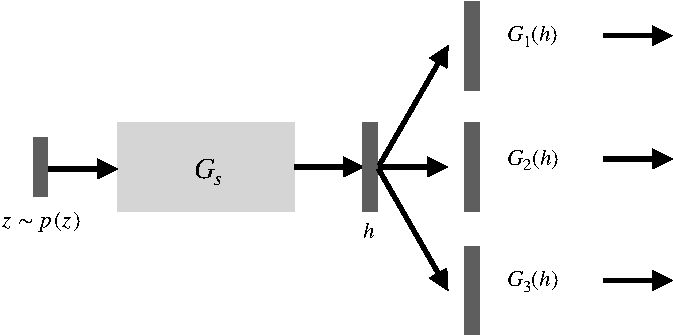
\includegraphics[width=0.75\columnwidth]{madgan.pdf}
\end{center}
\caption{Multi-agent diverse GAN}
\vskip\baselineskip % Leave a vertical skip below the figure
\label{fig:models:madgan}
\end{figure}

The model is shown in Figure \ref{fig:models:madgan}. Given $z$, a shared neural network block produces $z'$, an intermediate representation that is higher dimensional than $z$, which is used by a set of generators $\{G_i(z')\}_{i=1}^m$. The discriminator is a $m+1$-class classifier with 0 for true, and $1$ to $m$ for the fake instances. The discriminator should push the different generators to different modes to be able to solve the classification problem. More formally, the discriminator tries to minimize the following:
\begin{equation}
\min_{\phi} \quad -\mathbb{E}_{x \sim (p_t \cup p_f)} \left[ \sum_{j=0}^m r_j(x) \log D_j(x;\phi)\right]
\end{equation}
where $p_t$  and $p_f$ are the target and the fake distribution respectively, $r$ is a one-hot vector with $m+1$ length. This is the regular cross-entropy error function. The cost function for generators remains the same with a little twist that we try to minimize $\log (1 - D_0(x;\phi))$ instead of $\log (1 - D(x;\phi))$ since now $D_0$ represents the probability of $x$ coming from the true distribution.

Though there are multiple generators, we do not mix them in a co-operative manner. We also do not partition $p(z)$ and use each partition for different generators. This should rather be thought as each generator produces their own interpretation of $p(z)$. Therefore, instead of partitioning $p(z)$ we introduce alternative $p(z)$'s.
%
%
\section{Mixture GAN}
\label{sec:mgan}

MGAN \cite{hoang2018mgan} is similar to MAD-GAN except that the classifer and the discriminator are separate. The discriminator is two-class as usual discriminating between true and fake examples, and there is a separate $m$-class classifier only for the fake examples.

\begin{figure}[htbp]
\begin{center}
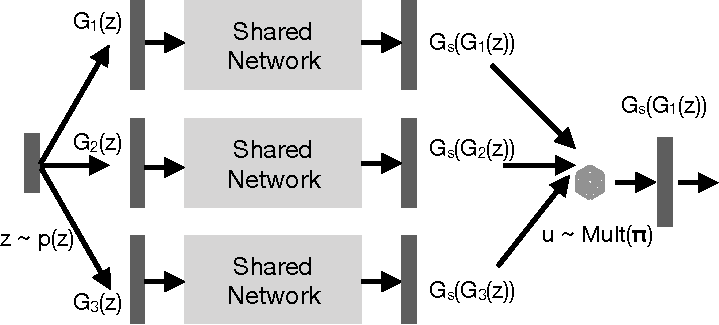
\includegraphics[width=0.75\columnwidth]{mgan.pdf}
\end{center}
\caption{Mixture GAN}
\vskip\baselineskip % Leave a vertical skip below the figure
\label{fig:models:mgan}
\end{figure}

The model is shown in Figure \ref{fig:models:mgan}. There is also the difference is that the split of the generators is earlier. A set of generators $\{G_i(z)\}_{i=1}^m$, transform $z$ and for all, the shared network $G_s$ produces the final output. A multinomial distribution is sampled to randomly select one of the generators. Parameters of the multinomial distribution are fixed. While the discriminator tries to discriminate between fake and real data as usual, the classifier tries to predict the index of the generator that produced the fake sample. These two networks share parameters treating discriminator/classifier as a multi-task learning problem. This approach also treats $p(z)$ as in MAD-GAN, creating alternative $p(z)$'s.

\section{Mixtures of Experts GAN}
\label{sec:megan}

In the MEGAN \cite{park2018megan}, inspired from the mixtures of experts \cite{jacobs1991adaptive}, there is an additional gating model, which is also trained, that chooses among the different generators.

\begin{figure}[htbp]
\begin{center}
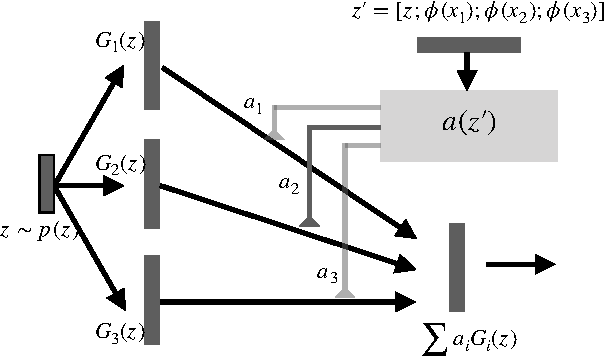
\includegraphics[width=0.75\columnwidth]{megan.pdf}
\end{center}
\caption{Mixture of experts GAN}
\vskip\baselineskip % Leave a vertical skip below the figure
\label{fig:models:megan}
\end{figure}

The model is shown in Figure \ref{fig:models:megan}. There is a set of generators $\{G_i(z)\}_{i=1}^{m}$ and an additional gating function, which takes as its input $z$ and some features from the generated $x$. Then Straight-Through Gumbel Softmax is applied which only selects one expert while allowing differentiability. The discriminator is still two-class. The gating model also has its parameters that are updated together with the generators. Although all generators generate an output, it is the gating model that decides which one is to be used. 

Different from MAD-GAN and MGAN, in this approach $p(z)$ is partitioned into local parts. Since there is a gating network, each generator is only responsible for a local part of $p(z)$. However, this partitioning is rather hard since we only let one generator to be used. Also, the gating network takes features from the generators' outputs as its input, therefore the partitioning might be non-smooth.

Many unsupervised learning methods assume that $x$ is determined by a set of factors $z$ and an unpredictable noise factor $\epsilon$. So instead of finding $p(x)$, we try to find $p(z)$ and the mapping between $p(z)$ and $p(x)$. In the GAN framework, we generally fix $p(z)$ to be a spherical Gaussian distribution and let $G$ to find the relation between $p(z)$ and $p(x)$. Since DNNs are very powerful function approximators, we hope that $G$ can map $p(z)$ to $p(x)$ even if we fix $p(z)$. However, this mapping might be arbitrarily hard. We instead propose to transform $p(z)$ at the earlier layers then use a shared network to generate the data. By this way, generator can decide how to transform $p(z)$. Also, we can analyze the $p(z)$ after the training to see the relation between clusters in $p(z)$.
%
%
\chapter{MIXTURES OF GENERATORS}
\label{chapter:mixture_gan}

\section{Mixtures of Experts}
\label{sec:me}
A mixture of experts (ME) model consists of local experts $\{f_i(x)\}_{i=1}^{m}$, and a gating function $g(x)$ \cite{jacobs1991adaptive}. Instead of learning a global function, we divide the input space into regions and learn a set of local functions. For a given input $x$, the gating function outputs probabilities that decide which experts to use. Each expert is responsible for modeling input-output mapping in its region. Experts can be simple models since each expert needs to learn a local input-output mapping instead of a global one. The formal definition of the model is as follows:
\begin{gather}
g(x) = \text{softmax}(W_g x + b_g)\\
y = \sum_{i=1}^m g_i(x) f_i(x)\\
\text{softmax}_i(x) = \frac{e^{x_i}}{\sum_j e^{x_j}}
\end{gather}
where $y$ is the response of the model. Experts can be any differentiable function. It is recommended that we keep experts simple since we employ a multiple of them. For example, this can be a constant response, $f_i(x)=\rho_i$, or a linear response, $f_i(x)=W_i x + b_i$.
%
\begin{figure}[htbp]
\begin{center}
\subfloat[Regression]{
	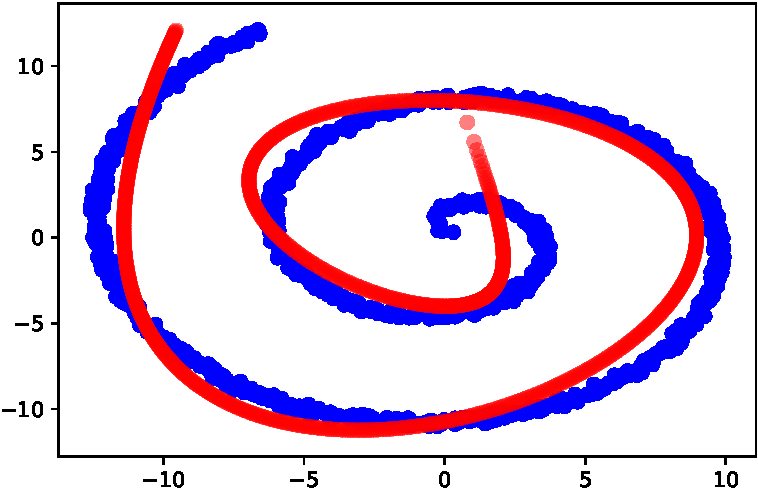
\includegraphics[width=0.5\linewidth]{me_regression.pdf}
	\label{fig:me:regression}
}
\subfloat[Cooperation]{
	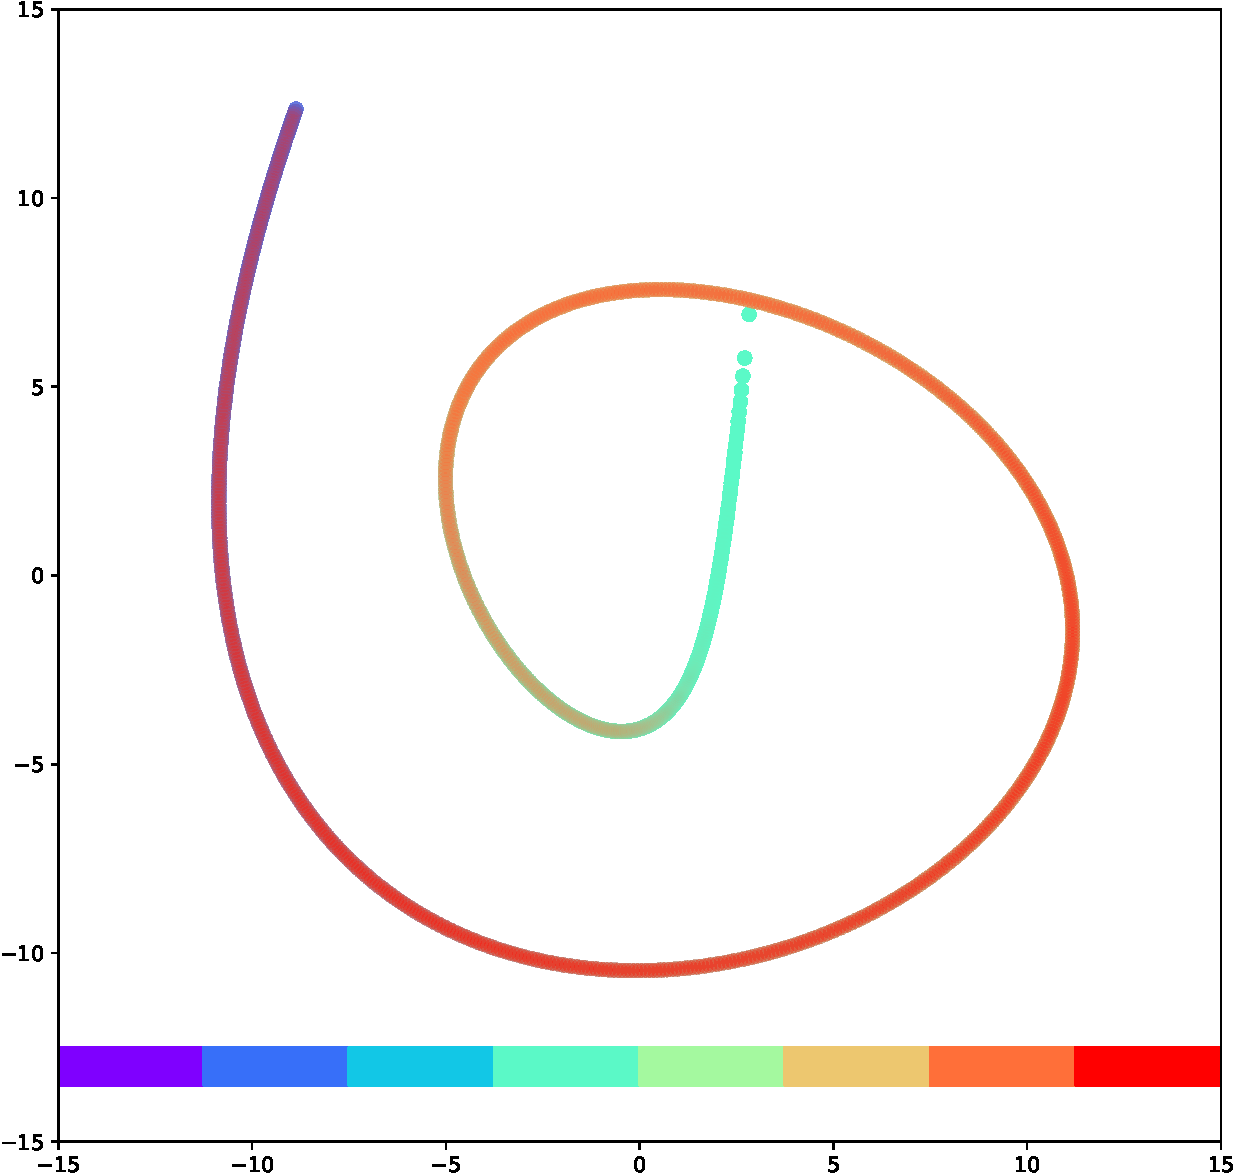
\includegraphics[width=0.5\linewidth]{me_coop.pdf}
	\label{fig:me:coop}
}

\subfloat[Experts]{
	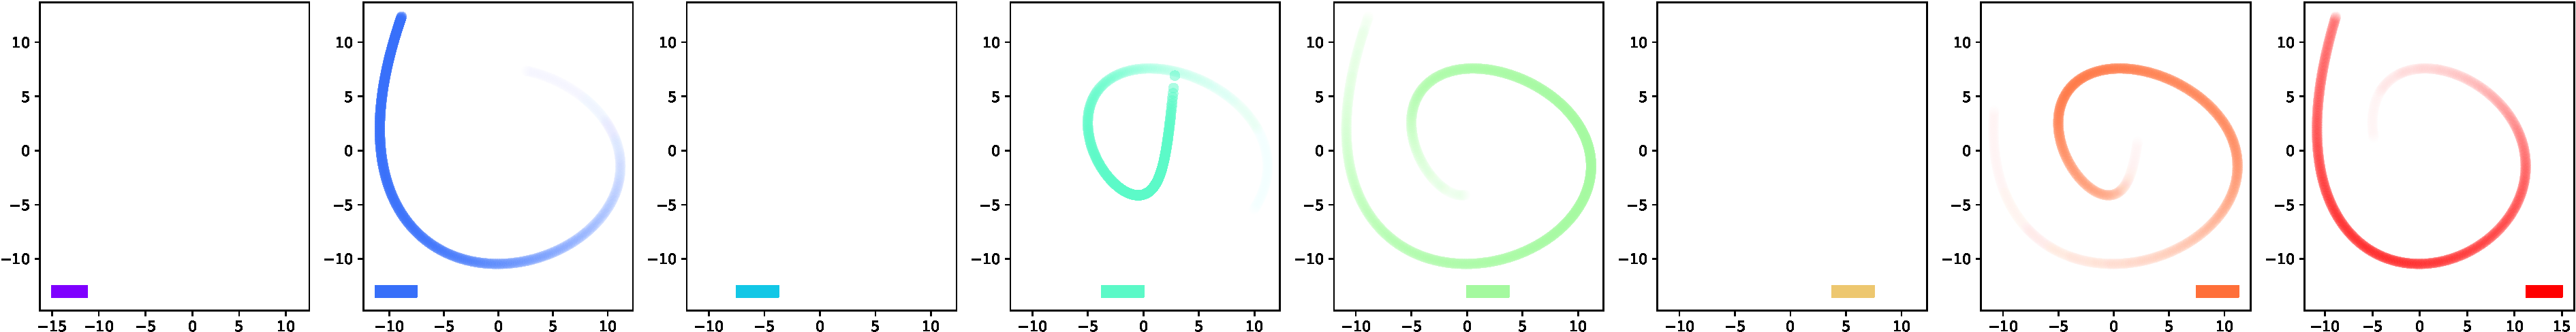
\includegraphics[width=\linewidth]{me_experts.pdf}
	\label{fig:me:experts}
}
\end{center}
\caption{Results of regression task on a spiral data set with a mixture of experts model.}
\vskip\baselineskip
\label{fig:me:model}
\end{figure}
%
For a visual understanding of the model, let us look at Figure \ref{fig:me:model}. We are given a spiral-like shaped two-dimensional data set. We trained an ME model with 8 linear experts. In Figure \ref{fig:me:regression}, we see the trained model's response. To see which expert is responsible for which part, we pick a color for each expert and visualize its response with the respective color. The responsibility of each expert is calculated by softly counting the gating function's output for each point. This soft count decides the transparency level (alpha level) of the visualized point. This is shown in Figure \ref{fig:me:coop}. The horizontal line in Figure \ref{fig:me:coop} shows the color of each expert. As we expect, we see that the color changes when we change the region. Responses of each expert alone is also shown in Figure \ref{fig:me:experts}. We understand that some experts are not used at all.

\section{Hierarchical Mixtures of Experts}
\label{sec:hme}
In hierarchical mixtures of experts model (HME) \cite{jordan1994hierarchical}, we define a tree structure where internal nodes contain gating functions and leaves contain experts. The difference between the ME model is that we replace the softmax gating function with a hierarchical mixture of sigmoid functions. The response of a binary tree node $m$ can be recursively defined as:
\begin{gather}
y_m(x)=
	\begin{cases}
		\hfil f_m(x) &\text{if $m$ is a leaf} \\
		\hfil y_m^{L}(x)g_m(x) + y_m^{R}(x)(1 - g_m(x)) &\text{otherwise}
	\end{cases}\\
g_m(x) = \frac{1}{1+e^{-(w_m x + b_m)}}
\end{gather}
where $y_m^L$ and $y_m^R$ are the responses of the left and the right children of node $m$ respectively. This can be also interpreted as a soft decision tree. In a hard decision tree, we either select the left child or the right child in a node whereas in a soft decision tree we take a convex combination of the child responses. One can fix the tree structure beforehand, or grow the tree adaptively based on the error \cite{irsoy2012soft,irsoy2014budding}. Since the whole model is continuous, we can use gradient based optimization to learn the model parameters.
%
\begin{figure}[htbp]
\begin{center}
\subfloat[Regression]{
	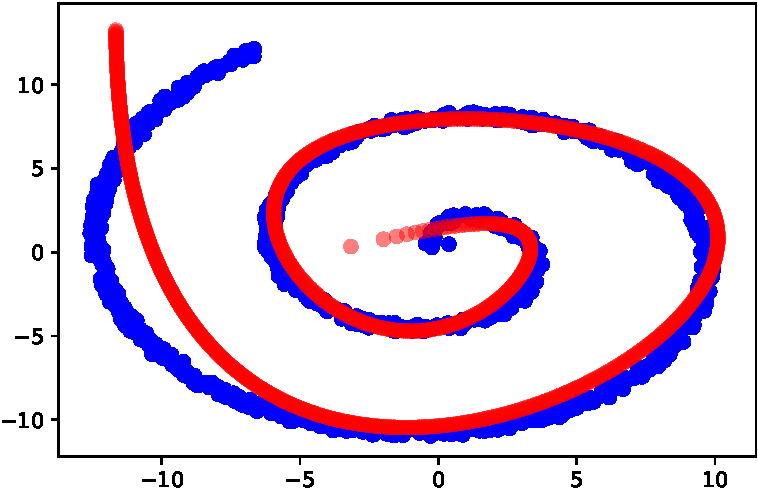
\includegraphics[width=0.5\linewidth]{hme_regression.pdf}
	\label{fig:hme:regression}
}
\subfloat[Cooperation]{
	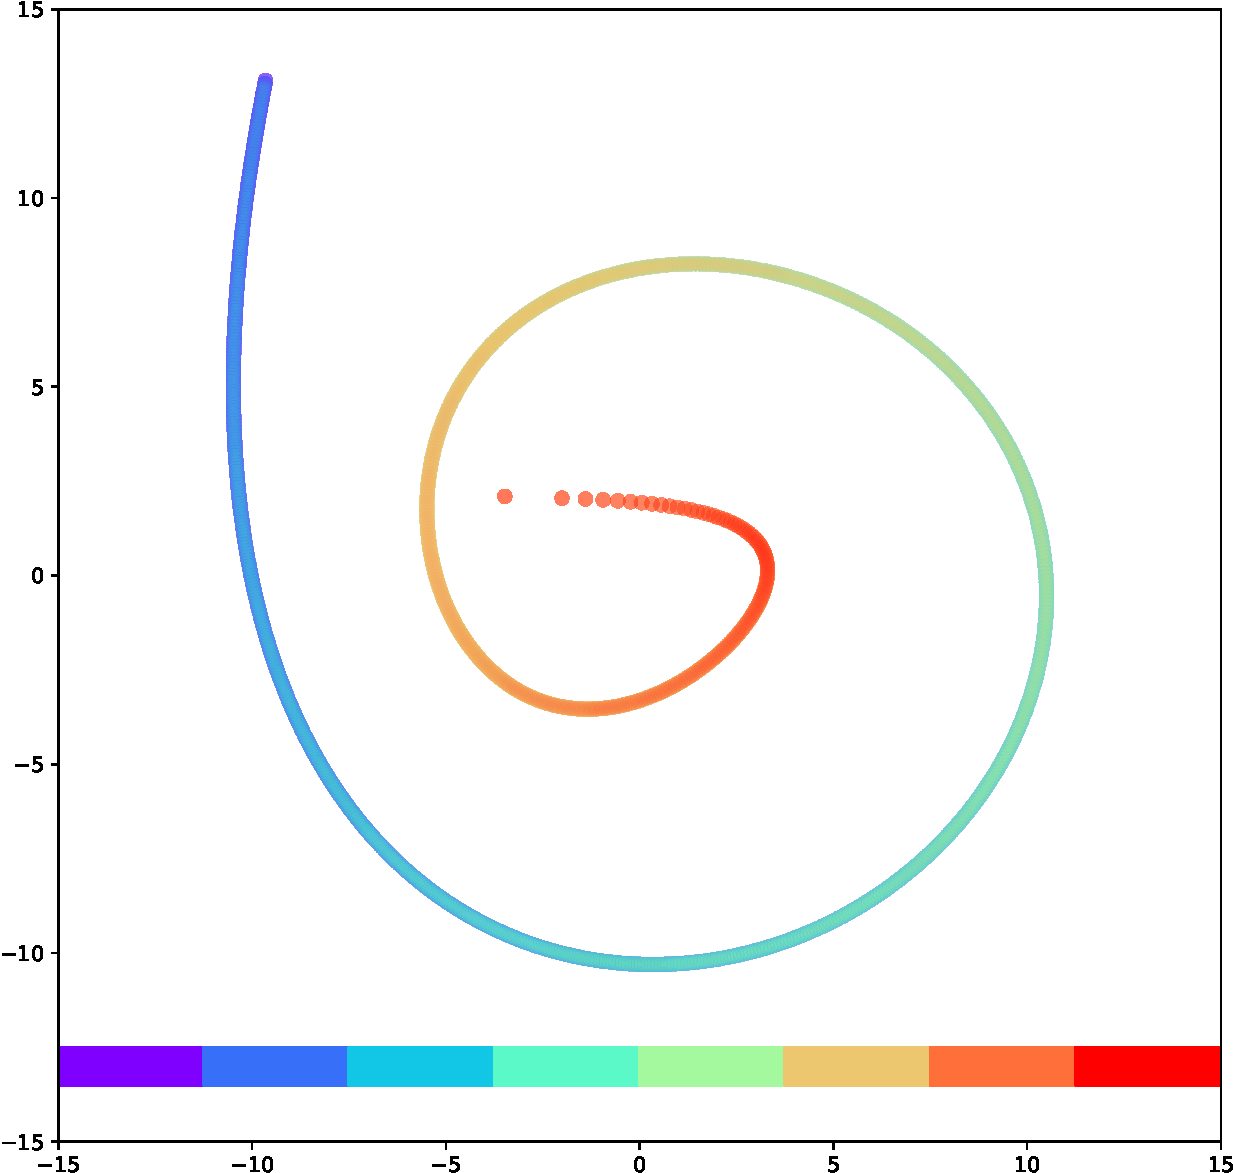
\includegraphics[width=0.5\linewidth]{hme_coop.pdf}
	\label{fig:hme:coop}
}

\subfloat[Experts]{
	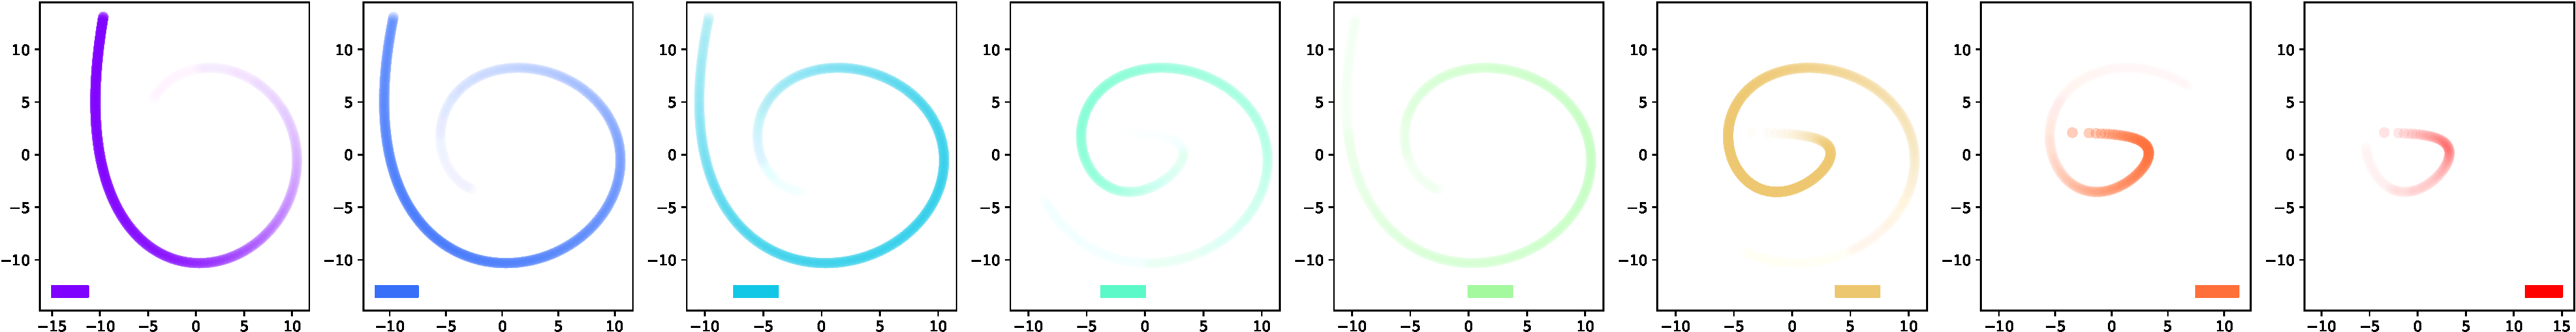
\includegraphics[width=\linewidth]{hme_experts.pdf}
	\label{fig:hme:experts}
}
\end{center}
\caption{Results of regression task on a spiral data set with a hierarchical mixture of experts model.}
\vskip\baselineskip
\label{fig:hme:model}
\end{figure}
%

The difference between HME and ME is the gating function. Note that given an input, each model takes a convex combination of their experts. However, the way this combination calculated is rather different. Because of the inherent tree structure of HME, experts that are children of the same parent are expected to have similar responses since the regions they are selected are closer. This brings such an interpretational advantage that we can understand the problem's procedural solution by looking at different levels of the tree. This will be further explained in later sections.

Let us now repeat the same experiment that we did in ME (Figure \ref{fig:hme:model}). We trained an HME model with a depth of 3 (therefore 8 experts). The response is quite the same. However, in Figure \ref{fig:hme:coop}, the curve is almost rainbow colored. In order for this to happen, each expert should be responsible of output, in the same order of color spectrum. This is shown more clearly in Figure \ref{fig:hme:experts}. In short, HME model first divides the spiral in half, use the left subtree for the outer region and the right subtree for the inner region. The same procedure is repeated for children (though the order may change).

\section{Flat Mixture of Generators}
\label{sec:flat_gen}
Our first proposed architecture uses mixtures of experts \cite{jacobs1991adaptive}. 

\section{Hierarchical Mixture of Generators}
\label{sec:hme_gen}

We propose the hierarchical mixture of generators, which learns a tree structure with internal decision nodes that divide up the input space and the leaves are local generators responsible from a local $z$ region generating a subset of $p(x)$. Since the splits are soft, given the tree structure, the parameters of the internal nodes as well as of the generators in the leaves can be updated using gradient-descent over Wasserstein loss. Note that it is only $G$ that is modeled this way, $D$ remains the usual deep neural network.

\begin{figure}[htbp]
\begin{center}
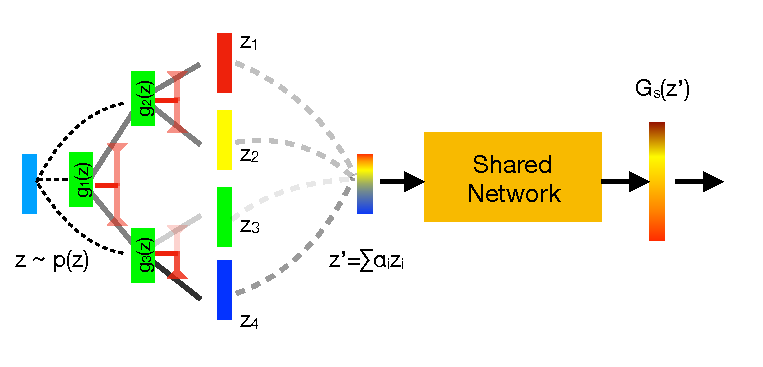
\includegraphics[width=0.75\columnwidth]{hmegan.pdf}
\end{center}
\caption{Hierarchical mixture of experts GAN}
\vskip\baselineskip % Leave a vertical skip below the figure
\label{fig:models:hmegan}
\end{figure}

% We use a widely adopted DCGAN \cite{radford2015unsupervised} architecture for the generator. In DCGAN, we project the input noise vector $\boldsymbol{z}$ into a high dimensional vector and reshape it to apply transposed convolution operation. This projection is done with a fully-connected perceptron layer. Here, we remove this layer and add a SDT. Given an input vector $\boldsymbol{z}$, SDT softly decides which leaves (experts) to use. Leaves contain high-dimensional vectors (to be used for transposed convolution), that are also learned throughout the training. The model is visually summarized in Figure \ref{fig:models:hmegan}. Instead of a tree structure, a flat gating function can also be used as in \cite{me}.
Just like the hierarchical mixture of experts \cite{jordan1994hierarchical} go from the flat organization of mixture of experts  \cite{jacobs1991adaptive} to a tree, our proposed hierarchical mixture of generators go from a flat mixture of generators to a tree. As shown in Figure \ref{fig:models:hmegan}, we have a binary tree where each internal node has a gating model that chooses between the two children based on $z$. The leaves of the tree give the output $\{z_i\}_{i=1}^m$. The final $z'$ is the weighted sum of all of the leaves weighted by the gating values on each path. A shared network then generates $x$ from this final $z'$.  We used the deconvolutional part of a widely used GAN architecture, namely DCGAN \cite{radford2015unsupervised}, as the shared network. Using a shared network is optional and depends on the domain we want to model. For image data sets, since images share lots of common texture, use of a shared network is essential for an economic (in terms of number of parameters) model.

Let $z \in \mathbb{R}^{d}$. In the original DCGAN architecture, the data lies in $\mathbb{R}^{d}$ after the first transformation even though the resulting vector is high-dimensional. When we use constant leaf vectors, HME can only output values in the \emph{convex hull} that is defined by its leaves since it takes a convex combination of its leaf vectors. Therefore, the data lies in $\mathbb{R}^m$ after the HME transformation where $m$ is the number of leaves. As a result, we separate the relation between the dimensionality of the input vector and the latent distribution. For example, we can set the dimensionality of the noise vector as $2$ but have a $128$-dimensional latent distribution that is defined by the output of the HME by using 128 leaves. The parameters of the gating functions and the leaves are learned throughout the training. The leaf values decide the vertices of the convex hull and the gating functions decide the distribution between the leaf values.

\chapter{EXPERIMENTS}
\label{chapter:exps}

\section{Data Sets}
\label{sec:datasets}
We test our proposed mixture model on five image data sets that are widely used in GAN literature: MNIST \cite{lecun1998mnist}, FashionMNIST \cite{xiao2017fashion}, CelebA \cite{liu2015deep},  UTZap50K \cite{yu2014fine} and Oxford Flowers (which we call ``Flowers'' in some tables to save for space) \cite{nilsback2008automated}.

MNIST is a data set that contains gray-scale handwritten digits of size $28 \times 28$ pixels. There are 60,000 training samples and 10,000 test samples.

FashionMNIST is a data set of fashion products such as t-shirts, trousers, sneakers. It is inspired from MNIST and has the same data structure with the same number of examples. It is designed to be a drop-in replacement from MNIST and known to be a harder baseline.

For these two data sets, we resize the images to $32 \times 32$ pixels, to be able to use the same kind of deconvolutional architecture repeatedly. We use all 10,000 examples in the test set for evaluation metrics.

CelebA contains colored celebrity faces with 40 different annotated features. There are 10,177 distinct people with a total of 202,599 images. We use the aligned-and-cropped version of the data set. There is no separate test set. We randomly select 10,000 test images and use it only in the evaluation. These images contain very different backgrounds therefore we further center-crop $148 \times 148$ pixels, and resize it to $64 \times 64$ pixels.

UTZap50K is a colored shoe data set of 50,000 catalog images. There are 4 major categories with many subcategories as brand names. We resize all images to $64 \times 64$. We randomly select 5,000 test images and use it only in the evaluation.

Oxford flowers is a colored flower data set with 102 different categories with a total of 8198 images. There are around 80 images per class. We resize all images to $64 \times 64$. We use 1,000 test images and use it only in the evaluation.

\begin{figure}[htbp]
\begin{center}
\subfloat[MNIST]{
	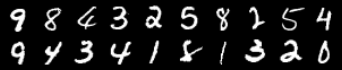
\includegraphics[width=0.5\linewidth]{mnist_dataset.png}
	\label{fig:dataset:mnist}
}
\subfloat[FashionMNIST]{
	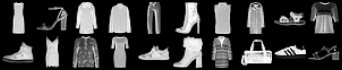
\includegraphics[width=0.5\linewidth]{fashion_dataset.png}
	\label{fig:dataset:fashion}
}

\subfloat[CelebA]{
	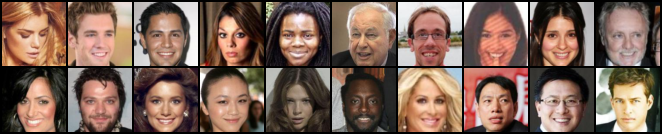
\includegraphics[width=0.5\linewidth]{celeba_dataset.png}
	\label{fig:dataset:celeba}
}
\subfloat[UTZap50K]{
	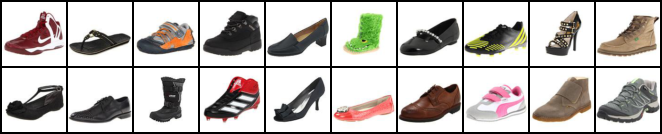
\includegraphics[width=0.5\linewidth]{utzap50k_dataset.png}
	\label{fig:dataset:utzap50k}
}

\subfloat[Oxford Flowers]{
	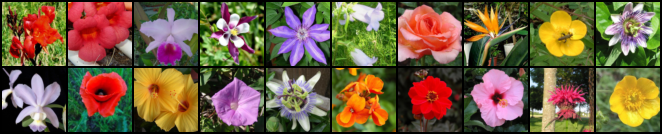
\includegraphics[width=0.5\linewidth]{flowers_dataset.png}
	\label{fig:dataset:flowers}
}
\end{center}
\caption{Samples from data sets.}
\vskip\baselineskip
\label{fig:datasets}
\end{figure}

Examples from each data set is shown in Figure \ref{fig:datasets}. All images contain pixel intensities in the range $[0, 255]$ as features. To improve training speed, we normalized all pixel intensities to range $[-1, 1]$. For MNIST and FashionMNIST, there are $32 \times 32=1024$ features. Other data sets are colored therefore there are three channels that describe red, green, blue pixel intensities. These have $64 \times 64 \times 3=12288$ features. 

\section{Experimental Setup}
\label{sec:setup}
These settings are applied to all experiments unless otherwise stated. The convolutional architecture that we use is the DCGAN \cite{radford2015unsupervised}. Since MNIST and FashionMNIST are $32\times 32$ pixels and other data sets are $64\times 64$ pixels, we used different networks with different sizes. The network architectures used for the former and latter data sets are given in Table \ref{tab:models} that shows the number of units in each layer and the convolutional structure. Layers 2 to 5 are transposed convolutional layers and layer 1 is fully connected for FC, or is where we have the HME or ME structure embedded. The dimensionality of the input $z$ is set to 100. We did not use normalization in $G$ but used layer normalization \cite{lei2016layer} in $D$.

\begin{table}[thbp]
\vskip\baselineskip
\caption{Deconvolution network architectures that are used. The small network is used on MNIST and FashionMNIST which are $32\times 32$ and the large is used on CelebA , UTZap50K and Oxford Flowers which are $64\times 64$.}
\begin{center}
\begin{tabular}{|l|c|c|}
\hline
\textbf{Layer} & \textbf{Small Network} & \textbf{Large Network}\\
 \hline
1 & 100                    & 100 \\
 \hline
2 &  $256 \times 4 \times 4$ & $512 \times 4 \times 4$\\
\hline
3 & $128 \times 8 \times 8$ & $256 \times 8 \times 8$\\
\hline
4 & $64 \times 16 \times 16$& $128 \times 16 \times 16$\\
 \hline
5 & $ 1 \times 32 \times 32$& $64 \times 32 \times 32$\\
 \hline
6 & - & $3 \times 64 \times 64$\\
 \hline
\end{tabular}
\label{tab:models}
\end{center}
\end{table}

Wasserstein loss \cite{arjovsky2017wasserstein} with gradient penalty \cite{gulrajani2017improved} is used. We adopted the suggested hyperparameter setting of Wasserstein loss recommended in \cite{gulrajani2017improved}, namely two-sided gradient penalty with a constant of $10.0$. The discriminator is trained 5 times per optimization step of the generator. We used Adam optimizer \cite{kingma2014adam} with amsgrad option \cite{reddi2019convergence}. Learning rate is set to $0.0001$ with beta values of Adam set to $(0.5, 0.999)$. We do not apply learning rate decay. Batch size is set to 128.

For the evaluation of GAN methods, we used the most popular evaluation criteria that are the Fr\'echet Inception distance (FID) \cite{heusel2017gans} and the two-sample test (C2ST) \cite{lopez2016revisiting}, here, 5-nearest neighbor (5-NN) leave-one-out accuracy. Both FID and 5-NN accuracy are calculated with the activations before the softmax layer (2048-dim) of InceptionV3 \cite{szegedy2016rethinking}. Lower FID scores are better and 5-NN accuracies that are close to 50\% are better. All models are run five times with different random seeds, and we report the average and standard deviations.

Seed numbers are set to {2019, 2020, 2021, 2022, 2023}. Except CuDNN \cite{chetlur2014cudnn} operations which are not deterministic but do not effect experiment results, all experiments are reproducible with given seeds. PyTorch auto-differentiation library \cite{paszke2017automatic} is used to automatically calculate gradients by exploiting the chain rule of Calculus. 

\section{Tree Structure vs. Flat Structure}
\label{sec:hme-vs-me}

First, we want to see whether there is a qualitative difference between the tree structure and the flat structure. We use trees of different depths, and we also test a flat mixture of generators of equal number of leaves. For example, we have a tree of depth five with 32 leaves and a flat mixture of 32 leaves. In the former case, for each leaf, we have five binary gatings; in the latter case, there is one gating that chooses one of 32. For the hierarchical model, we tested trees with depth 5, 6, 7 and 8. To get the same number of leaves, we used 32, 64, 128 and 256 generator experts in the flat mixture. These models are denoted as HME-$k$ and ME-$k$ respectively. We also report the parameter count of each model; these do not include the convolution parameters shared across all models.

\begin{table}[thbp]
\vskip\baselineskip
\caption[Results of FC and HME models]{Results of FC and HME models. $dim(\boldsymbol{z})$ is fixed to 100.}
\begin{center}
\begin{tabular}{|p{0.2cm}|p{0.2cm}|c|c|c|c|c|}
\cline{3-7}
\multicolumn{2}{c|}{} & FC		& HME-5		& HME-6		& HME-7		& HME-8		\\
\hline
\multirow{3}{*}{\rotatebox{90}{MNIST}}
& \rotatebox{90}{Real} & $74.90 \pm 0.59$ & $73.62 \pm 0.91^-$ & $73.70 \pm 0.54^-$ &  {$73.27 \pm 0.48^-$} &  {$73.39 \pm 0.47^-$} \\
\cline{2-7}
& \rotatebox{90}{Fake} & $67.89 \pm 0.30$ & $73.24 \pm 1.03^+$ & $72.00 \pm 1.10^+$ &  {$70.97 \pm 0.35^+$} &  {$71.20 \pm 0.48^+$} \\
\cline{2-7}
& \rotatebox{90}{FID} & $11.13 \pm 0.44$ & $13.57 \pm 0.31^+$ & $12.61 \pm 0.84^+$ & $11.93 \pm 0.44^+$ & {$11.84 \pm 0.48^+$} \\
\hline
\multicolumn{2}{|c|}{\#} & 413K & 134K & 268K & 537K & 1.07M \\
\hline
\multirow{3}{*}{\rotatebox{90}{Fashion}}
& \rotatebox{90}{Real} & $75.01 \pm 0.20$ & $73.46 \pm 0.68^-$ & $73.22 \pm 0.86^-$ & $73.14 \pm 1.47^-$ & $72.45 \pm 2.08$ \\
\cline{2-7}
& \rotatebox{90}{Fake} & $84.89 \pm 0.39$ & $89.32 \pm 0.72^+$ & {$88.36 \pm 0.95^+$} & {$87.47 \pm 1.14^+$} & {$86.95 \pm 1.27^+$} \\
\cline{2-7}
& \rotatebox{90}{FID} & $26.50 \pm 0.63$ & $27.92 \pm 0.91^+$ & $26.85 \pm 1.35$ & $25.93 \pm 1.48$ & {$25.51 \pm 2.41$} \\
\hline
\multicolumn{2}{|c|}{\#} & 413K & 134K & 268K & 537K & 1.07M \\
\hline
\multirow{3}{*}{\rotatebox{90}{CelebA}}
& \rotatebox{90}{Real} & $66.14 \pm 1.17$ & $72.16 \pm 0.51^+$ & $70.35 \pm 0.63^+$ & $68.61 \pm 0.81^+$ & $68.96 \pm 1.39^+$ \\
\cline{2-7}
& \rotatebox{90}{Fake} & $80.96 \pm 1.56$ & $91.14 \pm 0.40^+$ & $89.93 \pm 0.15^+$ & $87.71 \pm 0.95^+$ & $88.12 \pm 0.62^+$ \\
\cline{2-7}
& \rotatebox{90}{FID} & $14.93 \pm 0.48$ & $21.40 \pm 0.61^+$ & $19.97 \pm 0.27^+$ & $18.21 \pm 0.52^+$ & $18.20 \pm 0.47^+$ \\
\hline
\multicolumn{2}{|c|}{\#} & 827K & 265K & 530K & 1.06M & 2.12M \\
\hline
\multirow{3}{*}{\rotatebox{90}{UTZap50K}}
& \rotatebox{90}{Real} & $89.59 \pm 1.40$ & $91.64 \pm 0.83^+$ & $90.62 \pm 0.59$ & $90.47 \pm 0.70$ & $90.30 \pm 0.73$ \\
\cline{2-7}
& \rotatebox{90}{Fake} & $81.51 \pm 1.16$ & $86.02 \pm 0.67^+$ & $85.13 \pm 0.46^+$ & {$84.02 \pm 0.43^+$} & {$83.71 \pm 0.61^+$} \\
\cline{2-7}
& \rotatebox{90}{FID} & $54.48 \pm 5.36$ & $63.67 \pm 3.40^+$ & $58.96 \pm 1.28$ & $57.43 \pm 3.06$ & {$56.48 \pm 2.39$} \\
\hline
\multicolumn{2}{|c|}{\#} & 827K & 265K & 530K & 1.06M & 2.12M \\
\hline
\multirow{3}{*}{\rotatebox{90}{Flowers}}
& \rotatebox{90}{Real} & $93.80 \pm 1.02$ & $93.83 \pm 0.95$ & $93.41 \pm 0.96$ & $93.14 \pm 0.83$ & $93.38 \pm 0.96$ \\
\cline{2-7}
& \rotatebox{90}{Fake} & $97.60 \pm 0.71$ & $97.48 \pm 0.48$ & {$97.42 \pm 0.35$} & $97.46 \pm 0.58$ & $97.24 \pm 0.74$ \\
\cline{2-7}
& \rotatebox{90}{FID} & $135.28 \pm 7.28$ & $133.47 \pm 6.22$ & $131.05 \pm 4.61$ & $128.95 \pm 3.49$ & $128.62 \pm 5.94$ \\
\hline
\multicolumn{2}{|c|}{\#} & 827K & 265K & 530K & 1.06M & 2.12M \\
\hline
\end{tabular}
\label{tab:fc-hme}
\end{center}
\end{table}

\begin{table}[thbp]
\vskip\baselineskip
\caption[Results for ME models]{Results for ME models. $dim(\boldsymbol{z})$ is fixed to 100.}
\begin{center}
\begin{tabular}{|c|c|c|c|c|c|}
\cline{3-6}
\multicolumn{2}{c|}{} & ME-32		& ME-64		& ME-128		& ME-256 \\
\hline
\multirow{3}{*}{\rotatebox{90}{MNIST}}
& \rotatebox{90}{Real} & $74.23 \pm 0.58$ & $74.00 \pm 0.31^-$ & $74.57 \pm 0.86$ & $76.31 \pm 0.79^+$ \\
\cline{2-6}
& \rotatebox{90}{Fake} & $74.11 \pm 0.77^+$ & $72.12 \pm 0.74^+$ & $72.65 \pm 1.30^+$ & $72.97 \pm 0.52^+$ \\
\cline{2-6}
& \rotatebox{90}{FID} & $13.71 \pm 1.19^+$ & $12.08 \pm 0.23^+$ & $12.75 \pm 0.77^+$ & $14.58 \pm 1.10^+$ \\
\hline
\multicolumn{2}{|c|}{params.} & 134K & 268K & 537K & 1.07M \\
\hline
\multirow{3}{*}{\rotatebox{90}{Fashion}}
& \rotatebox{90}{Real} & $74.05 \pm 0.81$ & $73.54 \pm 1.10^-$ & $75.84 \pm 2.43$ & $75.63 \pm 2.48$ \\
\cline{2-6}
& \rotatebox{90}{Fake} & $90.23 \pm 0.47^+$ & $90.31 \pm 0.59^+$ & $90.50 \pm 1.47^+$ & $90.46 \pm 1.65^+$ \\
\cline{2-6}
& \rotatebox{90}{FID} & $27.68 \pm 0.83^+$ & $27.86 \pm 1.34$ & $28.47 \pm 2.90$ & $29.49 \pm 2.86$ \\
\hline
\multicolumn{2}{|c|}{params.} & 134K & 268K & 537K & 1.07M \\
\hline
\multirow{3}{*}{\rotatebox{90}{CelebA}}
& \rotatebox{90}{Real} & $72.22 \pm 1.60^+$ & $71.23 \pm 1.07^+$ & $69.66 \pm 0.84^+$ & $69.23 \pm 1.29^+$ \\
\cline{2-6}
& \rotatebox{90}{Fake} & $91.04 \pm 1.86^+$ & $90.56 \pm 1.87^+$ & $87.92 \pm 0.48^+$ & $87.83 \pm 0.66^+$ \\
\cline{2-6}
& \rotatebox{90}{FID} & $20.96 \pm 0.78^+$ & $20.27 \pm 0.70^+$ & $18.78 \pm 0.35^+$ & $18.39 \pm 0.76^+$ \\
\hline
\multicolumn{2}{|c|}{params.} & 265K & 530K & 1.06M & 2.12M \\
\hline
\multirow{3}{*}{\rotatebox{90}{UTZap50K}}
& \rotatebox{90}{Real} & $91.07 \pm 0.62$ & $91.18 \pm 0.34$ & $90.95 \pm 0.82$ & $91.31 \pm 1.18$ \\
\cline{2-6}
& \rotatebox{90}{Fake} & $86.69 \pm 1.18^+$ & $85.67 \pm 0.99^+$ & $85.38 \pm 0.42^+$ & $86.06 \pm 1.04^+$ \\
\cline{2-6}
& \rotatebox{90}{FID} & $63.72 \pm 4.35^+$ & $61.19 \pm 2.02^+$ & $61.51 \pm 2.52^+$ & $65.19 \pm 3.85^+$ \\
\hline
\multicolumn{2}{|c|}{params.} & 265K & 530K & 1.06M & 2.12M \\
\hline
\multirow{3}{*}{\rotatebox{90}{Flowers}}
& \rotatebox{90}{Real} & $93.58 \pm 1.26$ & $93.69 \pm 0.50$ & $93.57 \pm 1.41$ & $94.40 \pm 1.19$ \\
\cline{2-6}
& \rotatebox{90}{Fake} & $97.88 \pm 0.58$ & $97.96 \pm 0.30$ & $97.76 \pm 0.41$ & $97.89 \pm 0.48$ \\
\cline{2-6}
& \rotatebox{90}{FID} & $133.13 \pm 4.31$ & $131.83 \pm 2.45$ & $132.07 \pm 7.28$ & $137.08 \pm 6.46$ \\
\hline
\multicolumn{2}{|c|}{params.} & 265K & 530K & 1.06M & 2.12M \\
\hline
\end{tabular}
\label{tab:me}
\end{center}
\end{table}

Some samples generated from ME-64 and HME-6 are shown in Figure \ref{fig:samples} for visual inspection. It can be seen that these are quite realistic and contain diversity for both models. 5-NN and FID scores are given in Table \ref{tab:fc-hme} and \ref{tab:me} for HME and ME respectively. In general, it seems that they perform the same. From Table \ref{tab:fc-hme}, we see that the results for HME generally gets better with the increasing complexity (in terms of number of parameters) as expected. For ME (Table \ref{tab:me}), the results does not get better as in HME. Especially ME-256 model performs worse than other ME models with less parameters. We anticipate that more experts should bring more power. However, the gating function of ME does not get better when we increase the number of experts. Therefore, we conjecture that it is due to the gating function of ME, the results stagnates. However, this is not the case for HME since we distribute the gating function into many binary gating functions.

\begin{figure}[htbp]
\begin{center}
\subfloat[ME-64 leafs]{
	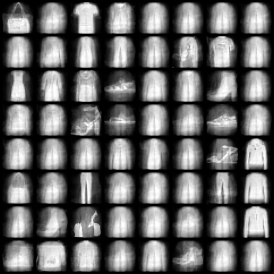
\includegraphics[width=0.5\linewidth]{me_leafs_fashion.png}
	\label{fig:leafs:me_fashion}
}
\subfloat[HME-6 leafs]{
	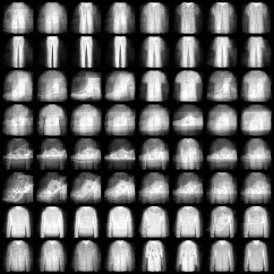
\includegraphics[width=0.5\linewidth]{hme_leafs_fashion.png}
	\label{fig:leafs:hme_fashion}
}
\end{center}
\caption{Leaf responsibilities of ME-64 (left) and HME-6 (right).}
\vskip\baselineskip
\label{fig:leafs}
\end{figure}

\begin{figure}[htbp]
\begin{center}
\subfloat{
	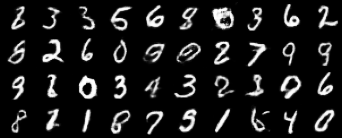
\includegraphics[width=0.5\linewidth]{me_samples_mnist.png}
	\label{fig:samples:me_mnist}
}
\subfloat{
	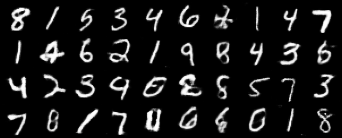
\includegraphics[width=0.5\linewidth]{hme_samples_mnist.png}
	\label{fig:samples:hme_mnist}
}

\subfloat{
	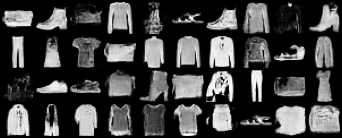
\includegraphics[width=0.5\linewidth]{me_samples_fashion.png}
	\label{fig:samples:me_fashion}
}
\subfloat{
	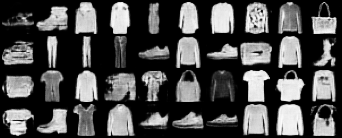
\includegraphics[width=0.5\linewidth]{hme_samples_fashion.png}
	\label{fig:samples:hme_fashion}
}

\subfloat{
	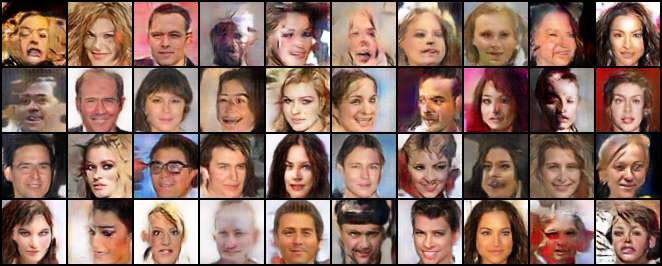
\includegraphics[width=0.5\linewidth]{me_samples_celeb.png}
	\label{fig:samples:me_celeb}
}
\subfloat{
	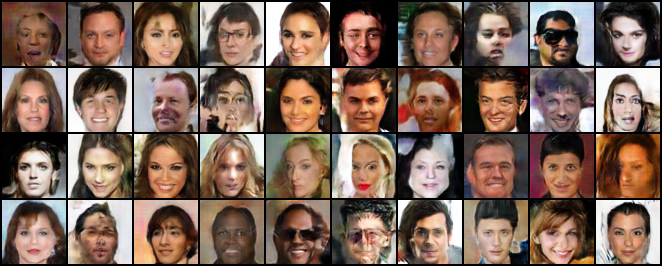
\includegraphics[width=0.5\linewidth]{hme_samples_celeb.png}
	\label{fig:samples:hme_celeb}
}

\subfloat{
	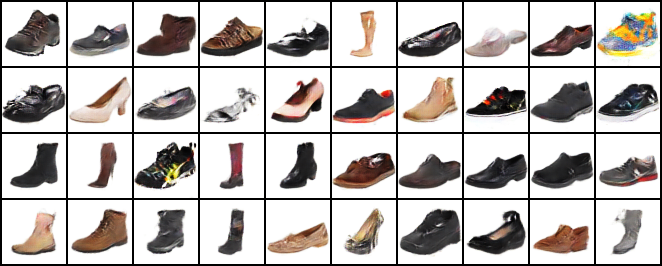
\includegraphics[width=0.5\linewidth]{me_samples_utzap50k.png}
	\label{fig:samples:me_utzap50k}
}
\subfloat{
	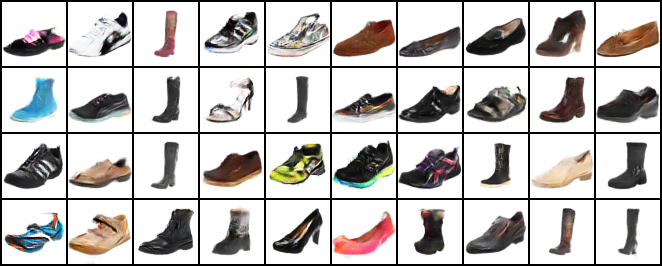
\includegraphics[width=0.5\linewidth]{hme_samples_utzap50k.png}
	\label{fig:samples:hme_utzap50k}
}

\subfloat{
	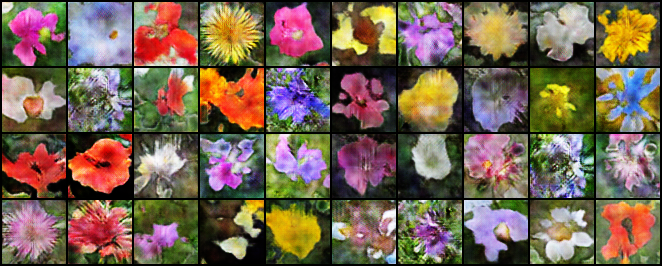
\includegraphics[width=0.5\linewidth]{me_samples_flowers.png}
	\label{fig:samples:me_flowers}
}
\subfloat{
	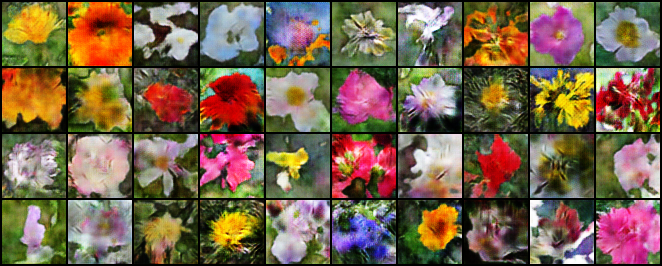
\includegraphics[width=0.5\linewidth]{hme_samples_flowers.png}
	\label{fig:samples:hme_flowers}
}
\end{center}
\caption{Samples generated using ME-64 (left) and HME-6 (right).}
\vskip\baselineskip
\label{fig:samples}
\end{figure}

We also tried to visualize the learned experts representations for ME and HME, as we did in Chapter \ref{chapter:mixture_gan}. To do this, we count the responsibility values (gating values) of leafs for each generated image. Then, for each leaf, we take a weighted average of generated images where weights are responsibilities of the leaf for each image. This will give us the leaf's expected responsibility, in other words its contribution. The result is shown in Figure \ref{fig:leafs}. We can say from the figure that HME leafs are more diverse and local when compared with ME leafs. Interpretation of this figure is important. This figure is not about sample quality or sample diversity. It is rather about the relation of leafs with each other. In Figure \ref{fig:leafs:me_fashion}, leafs seem more blurry. This says that leafs of ME are not specialized for a region of $p(z)$ but rather used throughout many regions of $p(z)$. To understand this clearly, we show the covariance matrices of leaf gating values in Figure \ref{fig:covariances}. These are $64 \times 64$ matrices where each index corresponds to a leaf. For example, for both matrices we see that the diagonal values are higher than others. This implies leafs are rather used alone, or used with high proportion. For ME in Figure \ref{fig:cov:me}, correlations are randomly scattered. Its counterpart HME (Figure \ref{fig:cov:hme}) has correlations gathered around the diagonal. Furthermore, we can see spectral squares of sizes $4 \times 4$ and $8 \times 8$. This shows that cooperations are done in a hierarchical way.

\begin{figure}[htbp]
\begin{center}
\subfloat[ME-64]{
	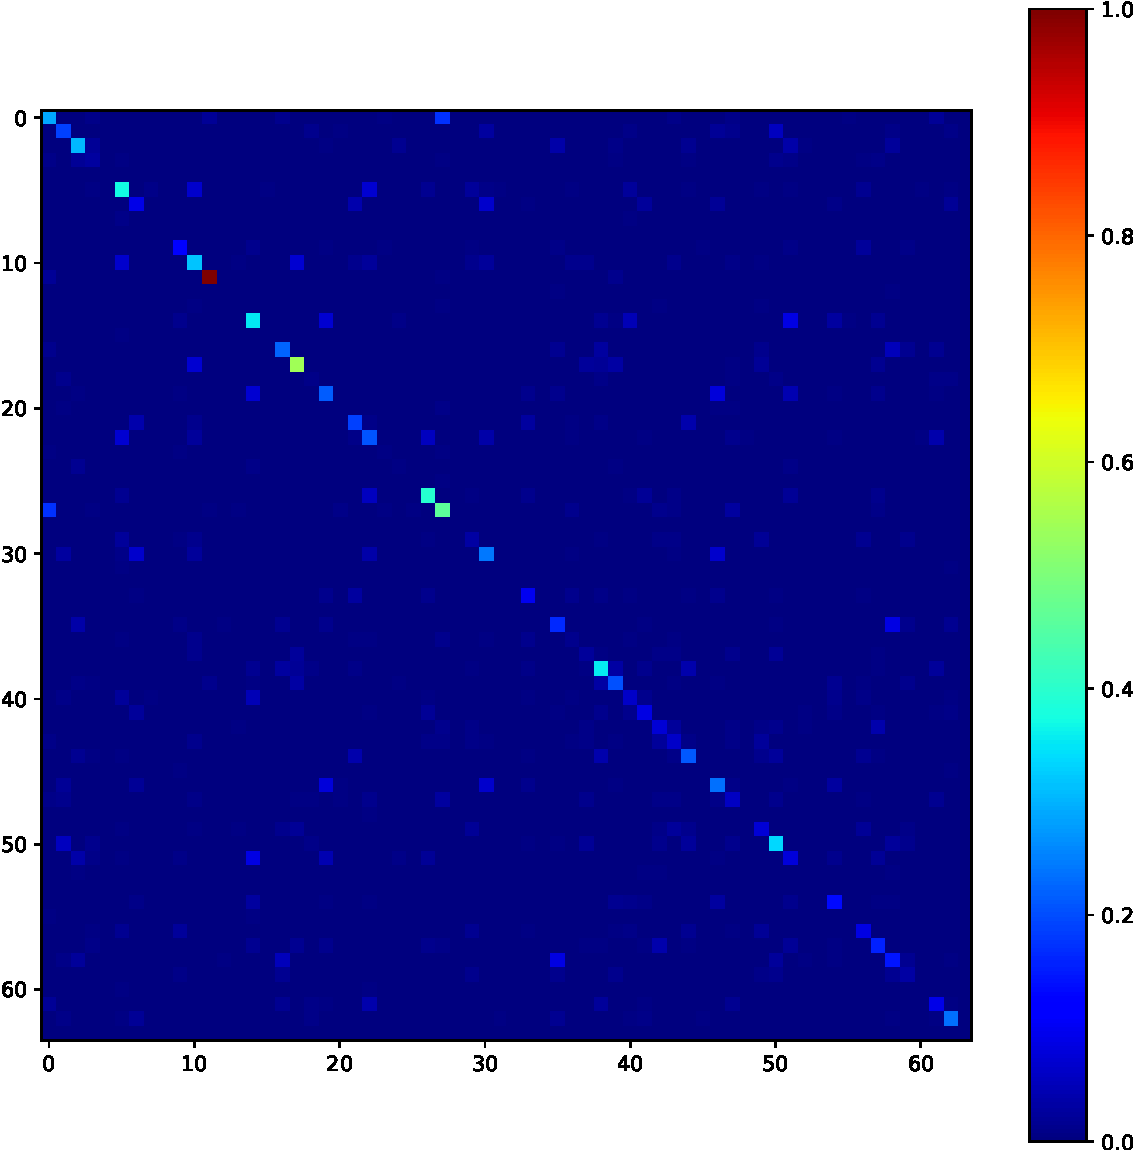
\includegraphics[width=0.5\linewidth]{cov_me.pdf}
	\label{fig:cov:me}
}
\subfloat[HME-6]{
	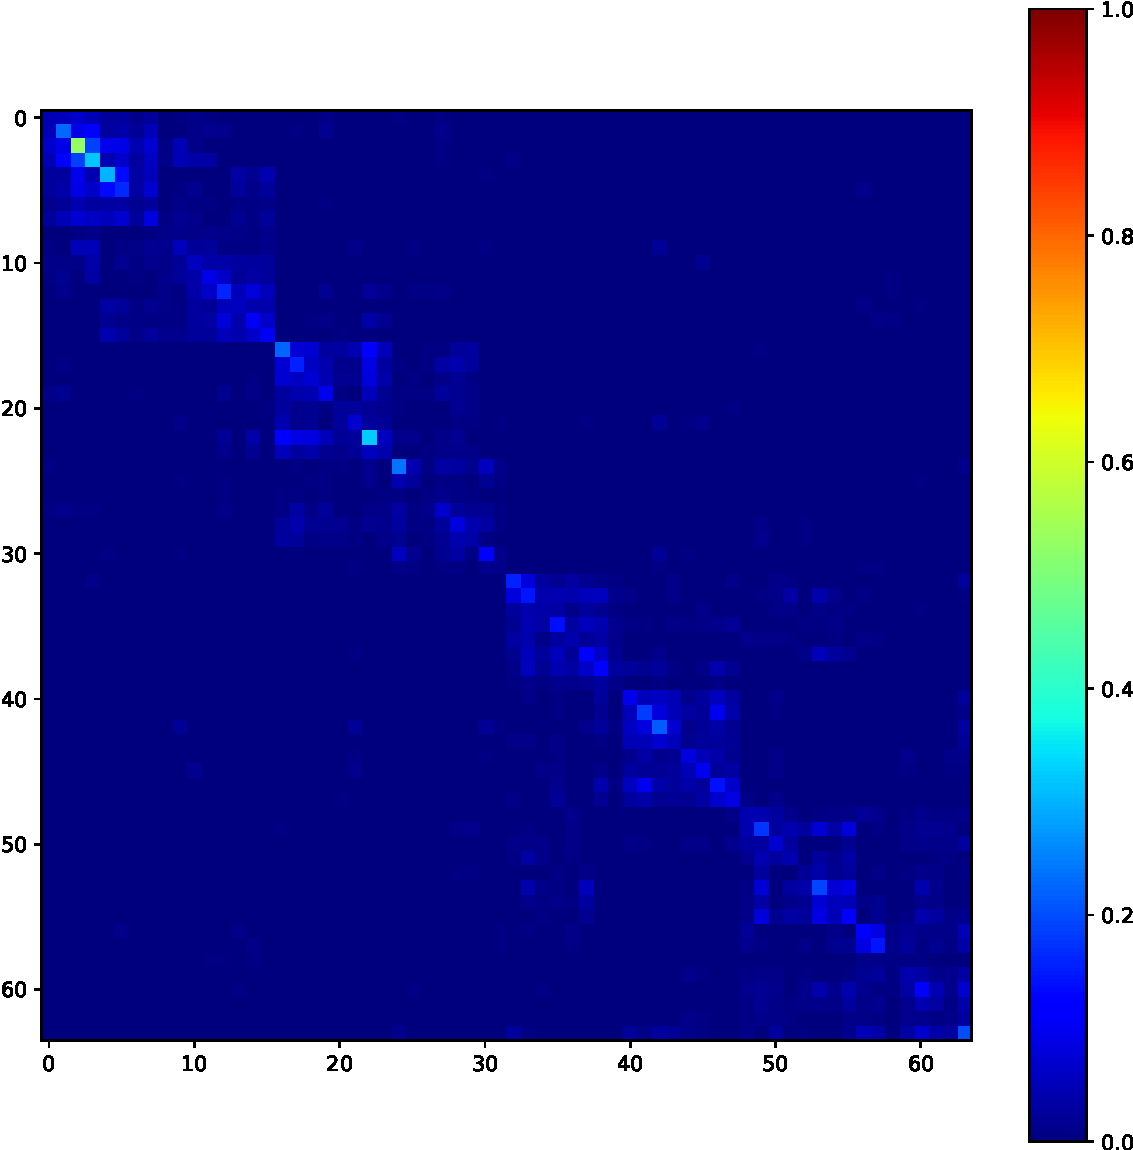
\includegraphics[width=0.5\linewidth]{cov_hme.pdf}
	\label{fig:cov:hme}
}
\end{center}
\caption{Covariance matrix of leaf densities for ME-64 and HME-6.}
\vskip\baselineskip
\label{fig:covariances}
\end{figure}

\section{Fully-connected vs. HME}
\label{sec:fc-vs-hme}
Now that we see the difference between ME and HME, we rather focus on HME and compare it with a fully-connected (FC) layer. In Figure \ref{fig:models:hmegan}, this corresponds to having one fully connected layer between $z$ and $z'$.

% One advantage of HME lies in complexity. Let us say $z$ is 100 dimensional and $z'$ is 1000 dimensional; a fully connected layer has 100,000 weights, but a tree uses gating nodes all of which are 100 dimensional, so unless the tree has more than 100 leaves, the tree is much simpler in terms of memory and computation.

Experiment results are reported in Table \ref{tab:fc-hme}. These results show that though HME is good, is not as good as FC in terms of FID score or 5-NN accuracy. Its performance improves as the structure gets larger; note that trees with depth 5 and 6 are smaller than FC. We conjecture that performance drop might be due to decreased sample diversity. Although 5-NN real accuracies are quite close, there is a gap between 5-NN fake accuracies. High 5-NN fake accuracy implies that fake samples are located near fake samples in $p(x)$.

One possible cause for the decreased diversity is to use constant vectors in the leafs. In FC version, the random vector $z$ is gone through an affine transformation and a rectified linear unit (ReLU) non-linearity. HME, on the other hand, encapsulates the information of $z$ in its gatings. Gating units are sigmoid functions. Sigmoid functions get saturated for values that are too low or too high. Therefore, if gating weights get too high or too low, which also means that it mimics a hard split instead of a soft one, the variety is lost due to sigmoid function. So although we want our experts to specialize, they output constant vectors when they are too specialized. To remedy this problem, we introduce linear experts in the leafs instead of constant vectors.

\section{Linear Experts}
\label{sec:hme-linear}

* leaflerin işlevleri *

* datayı hapsetme meselesi *

\begin{table}[thbp]
\vskip\baselineskip
\caption[HME with linear experts for different tree depths]{HME with linear experts for different tree depths. $dim(\boldsymbol{z})$ is fixed to 100. **welch's t-test yapılacak**}
\begin{center}
\begin{tabular}{|c|c|c|c|c|c|}
\hline
\multicolumn{2}{|c|}{Depth} & 2 & 3 & 4 & 5 \\
\hline
\multirow{3}{*}{\rotatebox{90}{MNIST}}
& \rotatebox{90}{Real} & $74.03 \pm 0.81$ & $73.48 \pm 0.53$ & $72.10 \pm 0.74$ & $72.14 \pm 0.54$ \\
\cline{2-6}
& \rotatebox{90}{Fake} & $66.73 \pm 0.61$ & $66.41 \pm 0.74$ & $66.21 \pm 0.82$ & $65.63 \pm 0.25$ \\
\cline{2-6}
& \rotatebox{90}{FID} & $10.27 \pm 0.41$ & $9.86 \pm 0.24$ & $9.15 \pm 0.45$ & $9.07 \pm 0.44$ \\
\hline
\multicolumn{2}{|c|}{params.} & 1.65M & 3.31M & 6.62M & 13.24M \\
\hline
\multirow{3}{*}{\rotatebox{90}{Fashion}}
& \rotatebox{90}{Real} & $72.18 \pm 0.38$ & $71.15 \pm 0.88$ & $70.08 \pm 0.84$ & $69.99 \pm 0.70$ \\
\cline{2-6}
& \rotatebox{90}{Fake} & $79.96 \pm 0.35$ & $79.14 \pm 0.73$ & $78.67 \pm 0.78$ & $78.10 \pm 0.60$ \\
\cline{2-6}
& \rotatebox{90}{FID} & $20.88 \pm 0.17$ & $19.64 \pm 0.89$ & $18.79 \pm 0.77$ & $18.24 \pm 0.91$ \\
\hline
\multicolumn{2}{|c|}{params.} & 1.65M & 3.31M & 6.62M & 13.24M \\
\hline
\multirow{3}{*}{\rotatebox{90}{CelebA}}
& \rotatebox{90}{Real} & $62.96 \pm 0.81$ & $63.15 \pm 1.42$ & $62.07 \pm 0.88$ & $62.02 \pm 1.02$ \\
\cline{2-6}
& \rotatebox{90}{Fake} & $77.91 \pm 0.83$ & $77.68 \pm 1.91$ & $77.18 \pm 0.82$ & $77.02 \pm 0.98$ \\
\cline{2-6}
& \rotatebox{90}{FID} & $12.41 \pm 0.40$ & $12.48 \pm 0.65$ & $12.23 \pm 0.56$ & $12.09 \pm 0.56$ \\
\hline
\multicolumn{2}{|c|}{params.} & 3.30M & 6.61M & 13.23M & 26.47M \\
\hline
\multirow{3}{*}{\rotatebox{90}{UTZap50K}}
& \rotatebox{90}{Real} & $87.26 \pm 0.80$ & $87.39 \pm 0.96$ & $87.61 \pm 1.21$ & $87.77 \pm 1.17$ \\
\cline{2-6}
& \rotatebox{90}{Fake} & $77.46 \pm 1.09$ & $78.21 \pm 0.32$ & $78.10 \pm 0.43$ & $78.42 \pm 1.36$ \\
\cline{2-6}
& \rotatebox{90}{FID} & $42.35 \pm 3.27$ & $42.99 \pm 2.08$ & $44.88 \pm 3.48$ & $45.54 \pm 3.46$ \\
\hline
\multicolumn{2}{|c|}{params.} & 3.30M & 6.61M & 13.23M & 26.47M \\
\hline
\multirow{3}{*}{\rotatebox{90}{Flowers}}
& \rotatebox{90}{Real} & $88.96 \pm 0.93$ & $89.30 \pm 1.49$ & $88.89 \pm 1.51$ & $90.15 \pm 1.60$ \\
\cline{2-6}
& \rotatebox{90}{Fake} & $96.58 \pm 0.58$ & $96.43 \pm 0.65$ & $96.61 \pm 0.41$ & $96.55 \pm 0.76$ \\
\cline{2-6}
& \rotatebox{90}{FID} & $111.06 \pm 4.84$ & $111.85 \pm 3.65$ & $112.78 \pm 3.13$ & $114.79 \pm 4.20$ \\
\hline
\multicolumn{2}{|c|}{params.} & 3.30M & 6.61M & 13.23M & 26.47M \\
\hline
\end{tabular}
\label{tab:hme-depth}
\end{center}
\end{table}

\begin{table}[thbp]
\vskip\baselineskip
\caption[ME with linear experts for different number of experts]{ME with linear experts for different number of experts. $dim(\boldsymbol{z})$ is fixed to 100. **welch's t-test yapılacak**}
\begin{center}
\begin{tabular}{|c|c|c|c|c|c|}
\hline
\multicolumn{2}{|c|}{Depth} & 4 & 8 & 16 & 32 \\
\hline
\multirow{3}{*}{\rotatebox{90}{MNIST}}
& \rotatebox{90}{Real} & $72.91 \pm 0.93$ & $71.46 \pm 1.02$ & $70.91 \pm 0.83$ & x \\
\cline{2-6}
& \rotatebox{90}{Fake} & $66.29 \pm 0.97$ & $66.25 \pm 0.72$ & $65.38 \pm 0.70$ & x \\
\cline{2-6}
& \rotatebox{90}{FID} & $9.74 \pm 0.64$ & $8.95 \pm 0.28$ & $8.56 \pm 0.53$ & x \\
\hline
\multicolumn{2}{|c|}{params.} & 1.65M & 3.31M & 6.62M & 13.24M \\
\hline
\multirow{3}{*}{\rotatebox{90}{Fashion}}
& \rotatebox{90}{Real} & $72.28 \pm 0.60$ & $70.90 \pm 0.96$ & $69.45 \pm 0.71$ & x \\
\cline{2-6}
& \rotatebox{90}{Fake} & $79.81 \pm 0.93$ & $78.64 \pm 0.51$ & $78.09 \pm 0.73$ & x \\
\cline{2-6}
& \rotatebox{90}{FID} & $20.90 \pm 0.87$ & $19.37 \pm 0.90$ & $18.09 \pm 0.89$ & x \\
\hline
\multicolumn{2}{|c|}{params.} & 1.65M & 3.31M & 6.62M & 13.24M \\
\hline
\multirow{3}{*}{\rotatebox{90}{CelebA}}
& \rotatebox{90}{Real} & x & $61.44 \pm 1.27$ & $62.63 \pm 0.67$ & $63.01 \pm 1.08$ \\
\cline{2-6}
& \rotatebox{90}{Fake} & x & $77.36 \pm 0.50$ & $78.11 \pm 0.96$ & $77.74 \pm 1.31$ \\
\cline{2-6}
& \rotatebox{90}{FID} & x & $11.99 \pm 0.27$ & $12.41 \pm 0.45$ & $12.64 \pm 0.63$ \\
\hline
\multicolumn{2}{|c|}{params.} & 3.30M & 6.61M & 13.23M & 26.47M \\
\hline
\multirow{3}{*}{\rotatebox{90}{UTZap50K}}
& \rotatebox{90}{Real} & $87.30 \pm 1.27$ & $86.83 \pm 1.12$ & $86.97 \pm 0.54$ & $87.68 \pm 0.76$ \\
\cline{2-6}
& \rotatebox{90}{Fake} & $77.82 \pm 1.40$ & $77.25 \pm 1.53$ & $77.50 \pm 1.13$ & $77.96 \pm 0.68$ \\
\cline{2-6}
& \rotatebox{90}{FID} & $43.05 \pm 3.83$ & $41.95 \pm 2.82$ & $41.45 \pm 1.99$ & $44.80 \pm 2.39$ \\
\hline
\multicolumn{2}{|c|}{params.} & 3.30M & 6.61M & 13.23M & 26.47M \\
\hline
\multirow{3}{*}{\rotatebox{90}{Flowers}}
& \rotatebox{90}{Real} & $89.25 \pm 2.64$ & $88.59 \pm 1.43$ & $89.33 \pm 1.39$ & $90.12 \pm 1.17$ \\
\cline{2-6}
& \rotatebox{90}{Fake} & $96.84 \pm 0.85$ & $96.79 \pm 0.69$ & $96.93 \pm 0.36$ & $97.11 \pm 0.80$ \\
\cline{2-6}
& \rotatebox{90}{FID} & $112.05 \pm 6.88$ & $113.37 \pm 3.92$ & $115.45 \pm 3.02$ & $118.00 \pm 4.52$ \\
\hline
\multicolumn{2}{|c|}{params.} & 3.30M & 6.61M & 13.23M & 26.47M \\
\hline
\end{tabular}
\label{tab:me-depth}
\end{center}
\end{table}

\section{Interpretation of the Learned Model}
\label{sec:interpret}
Though our proposed model is not as good as the FC in terms of FID or 5-NN scores, its main advantage is interpretability. To investigate the learned representation, we generate $100$ samples from the generated model and for each node $m$, we take a weighted average of the generated samples. In a hard decision tree where we choose left or right, a hard count corresponds to the path from root to prediction leaf. Here, we instead find the soft count of a node by multiplying the gating values up to that node. The result is visualized in Figure \ref{fig:polar:mnist}. We see that earlier levels of the tree correspond to the means of larger samples and as we go down to the leaves, there is specialization, an indication that the tree structure divides the input space into regions. We can think of the structure implementing a soft hierarchical clustering. 

\begin{figure}[htbp]
\begin{center}
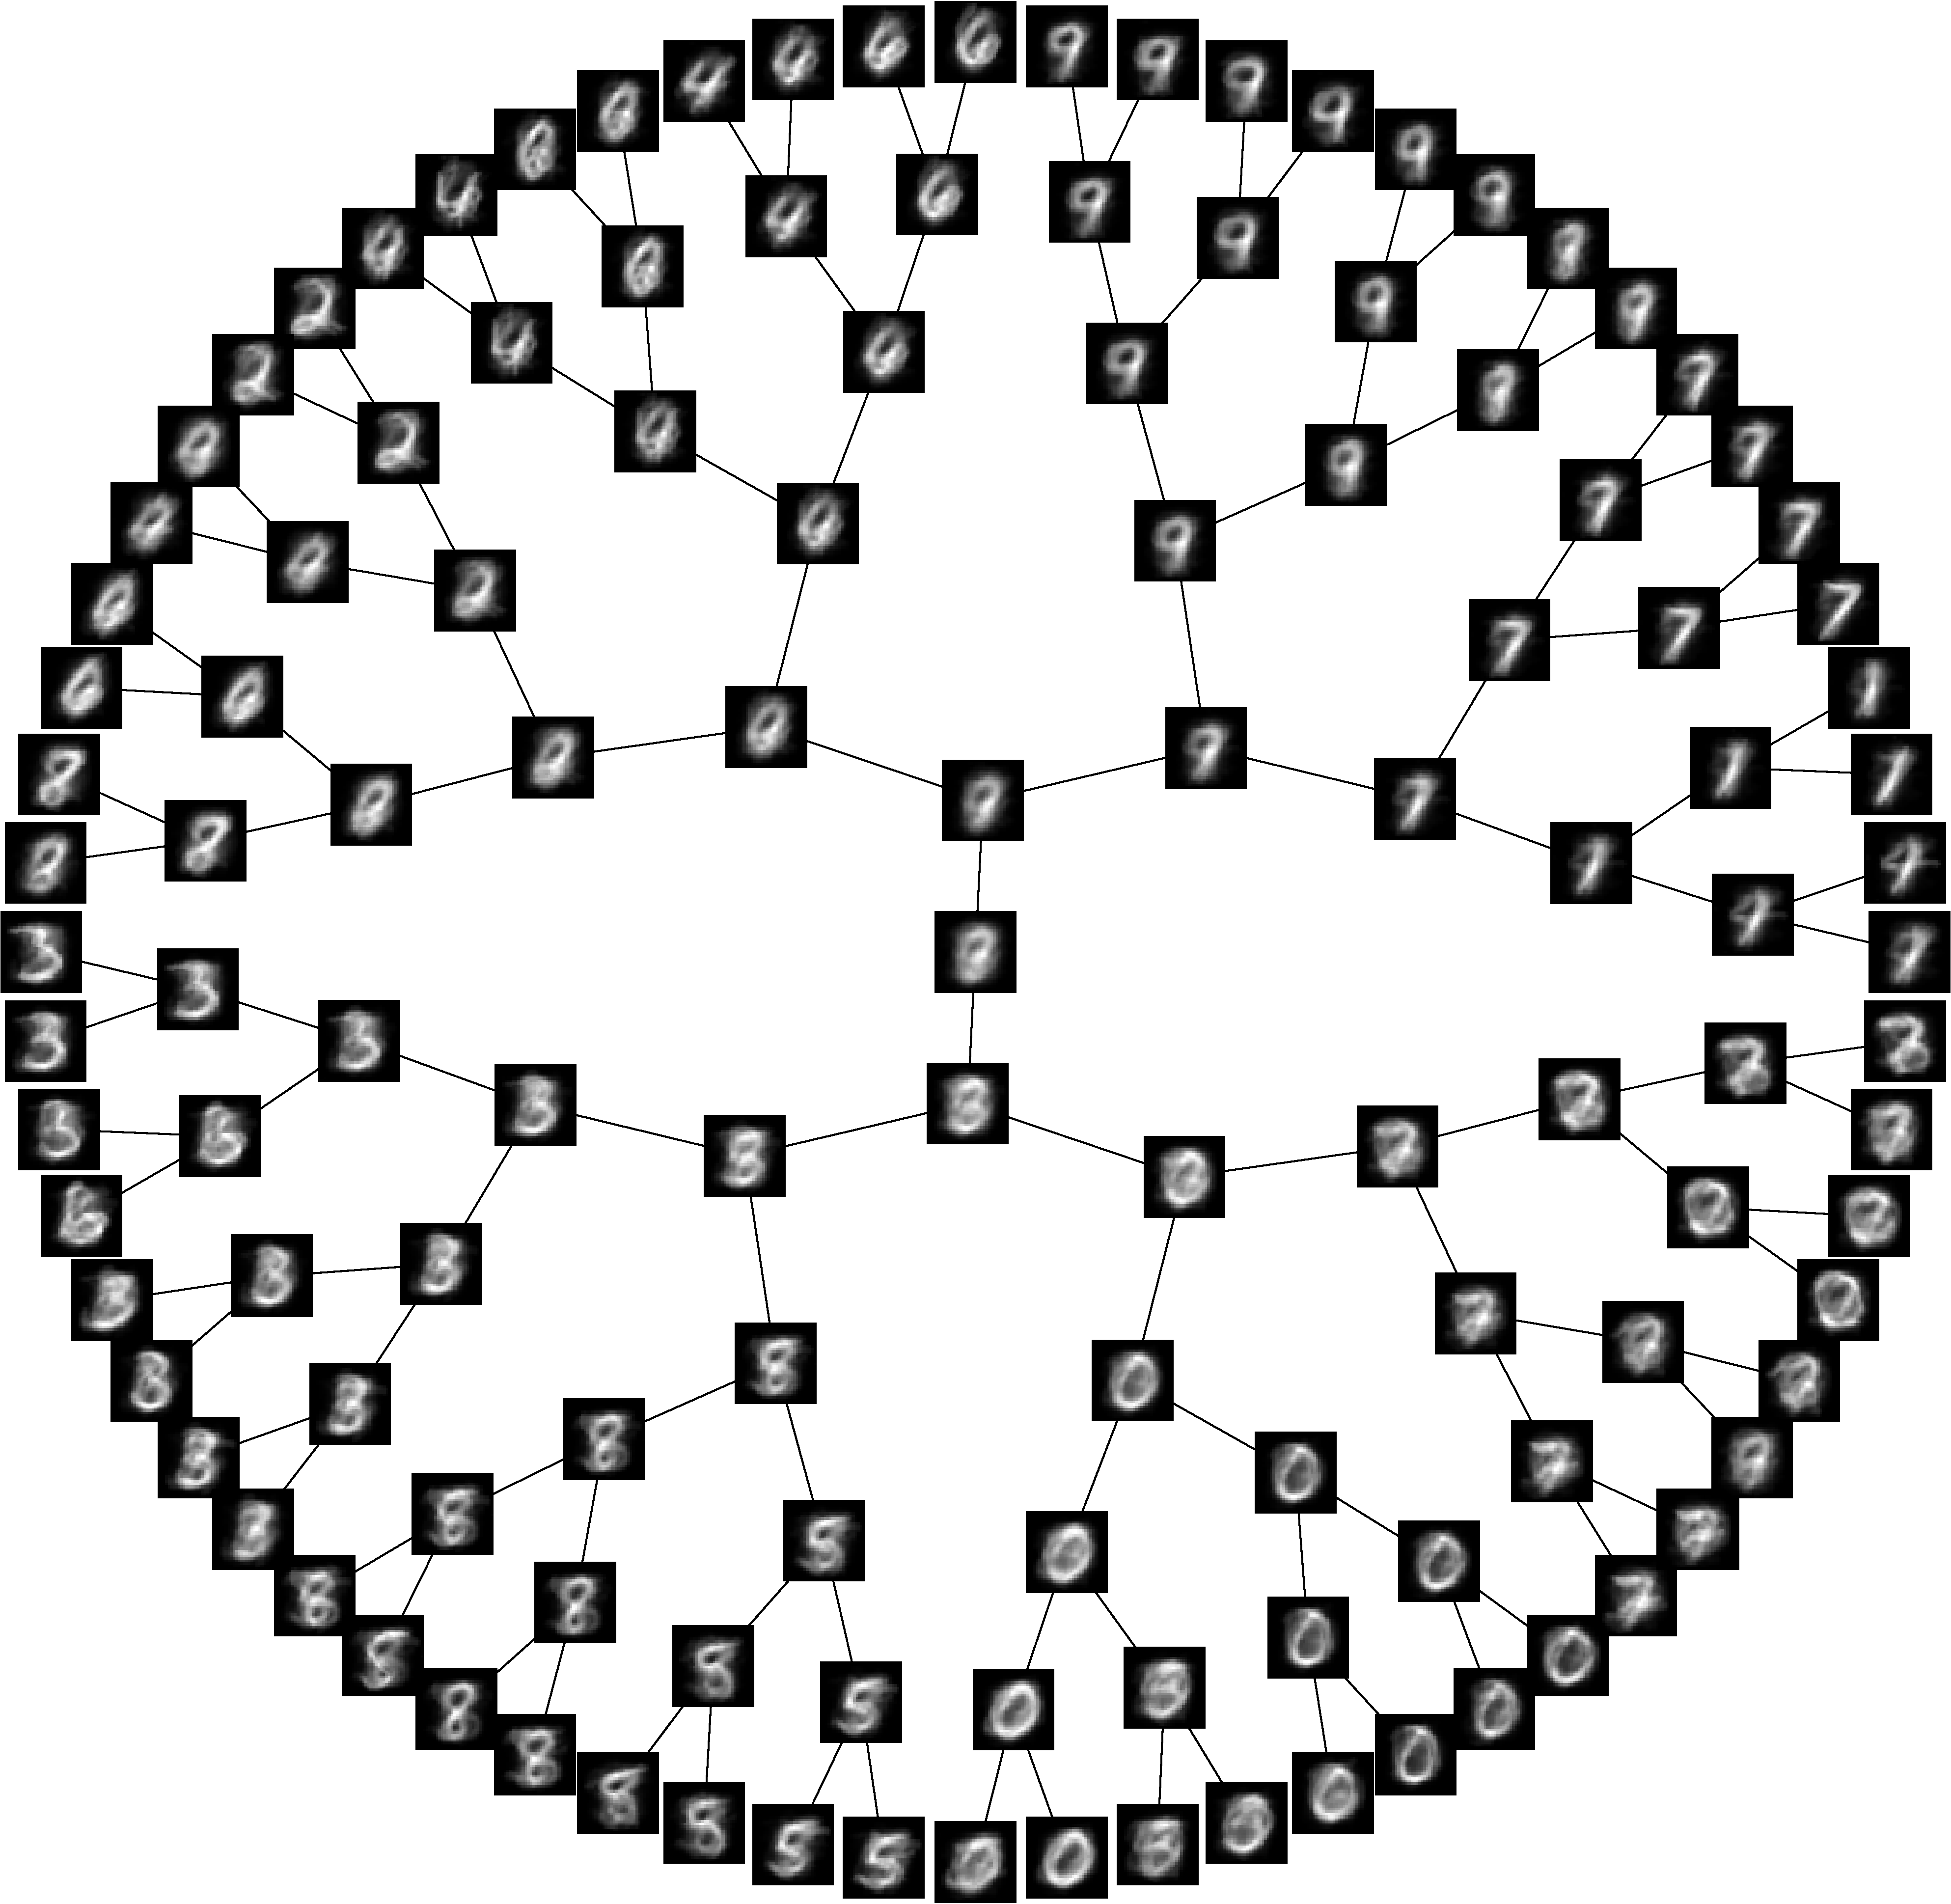
\includegraphics[width=\columnwidth]{polar_mnist.pdf}
\end{center}
\caption{Mean responses of each node. At the center, there is the root. As we go outer, the depth increases and therefore granularity level increases.}
\vskip\baselineskip % Leave a vertical skip below the figure
\label{fig:polar:mnist}
\end{figure}

\begin{figure}[htbp]
\begin{center}
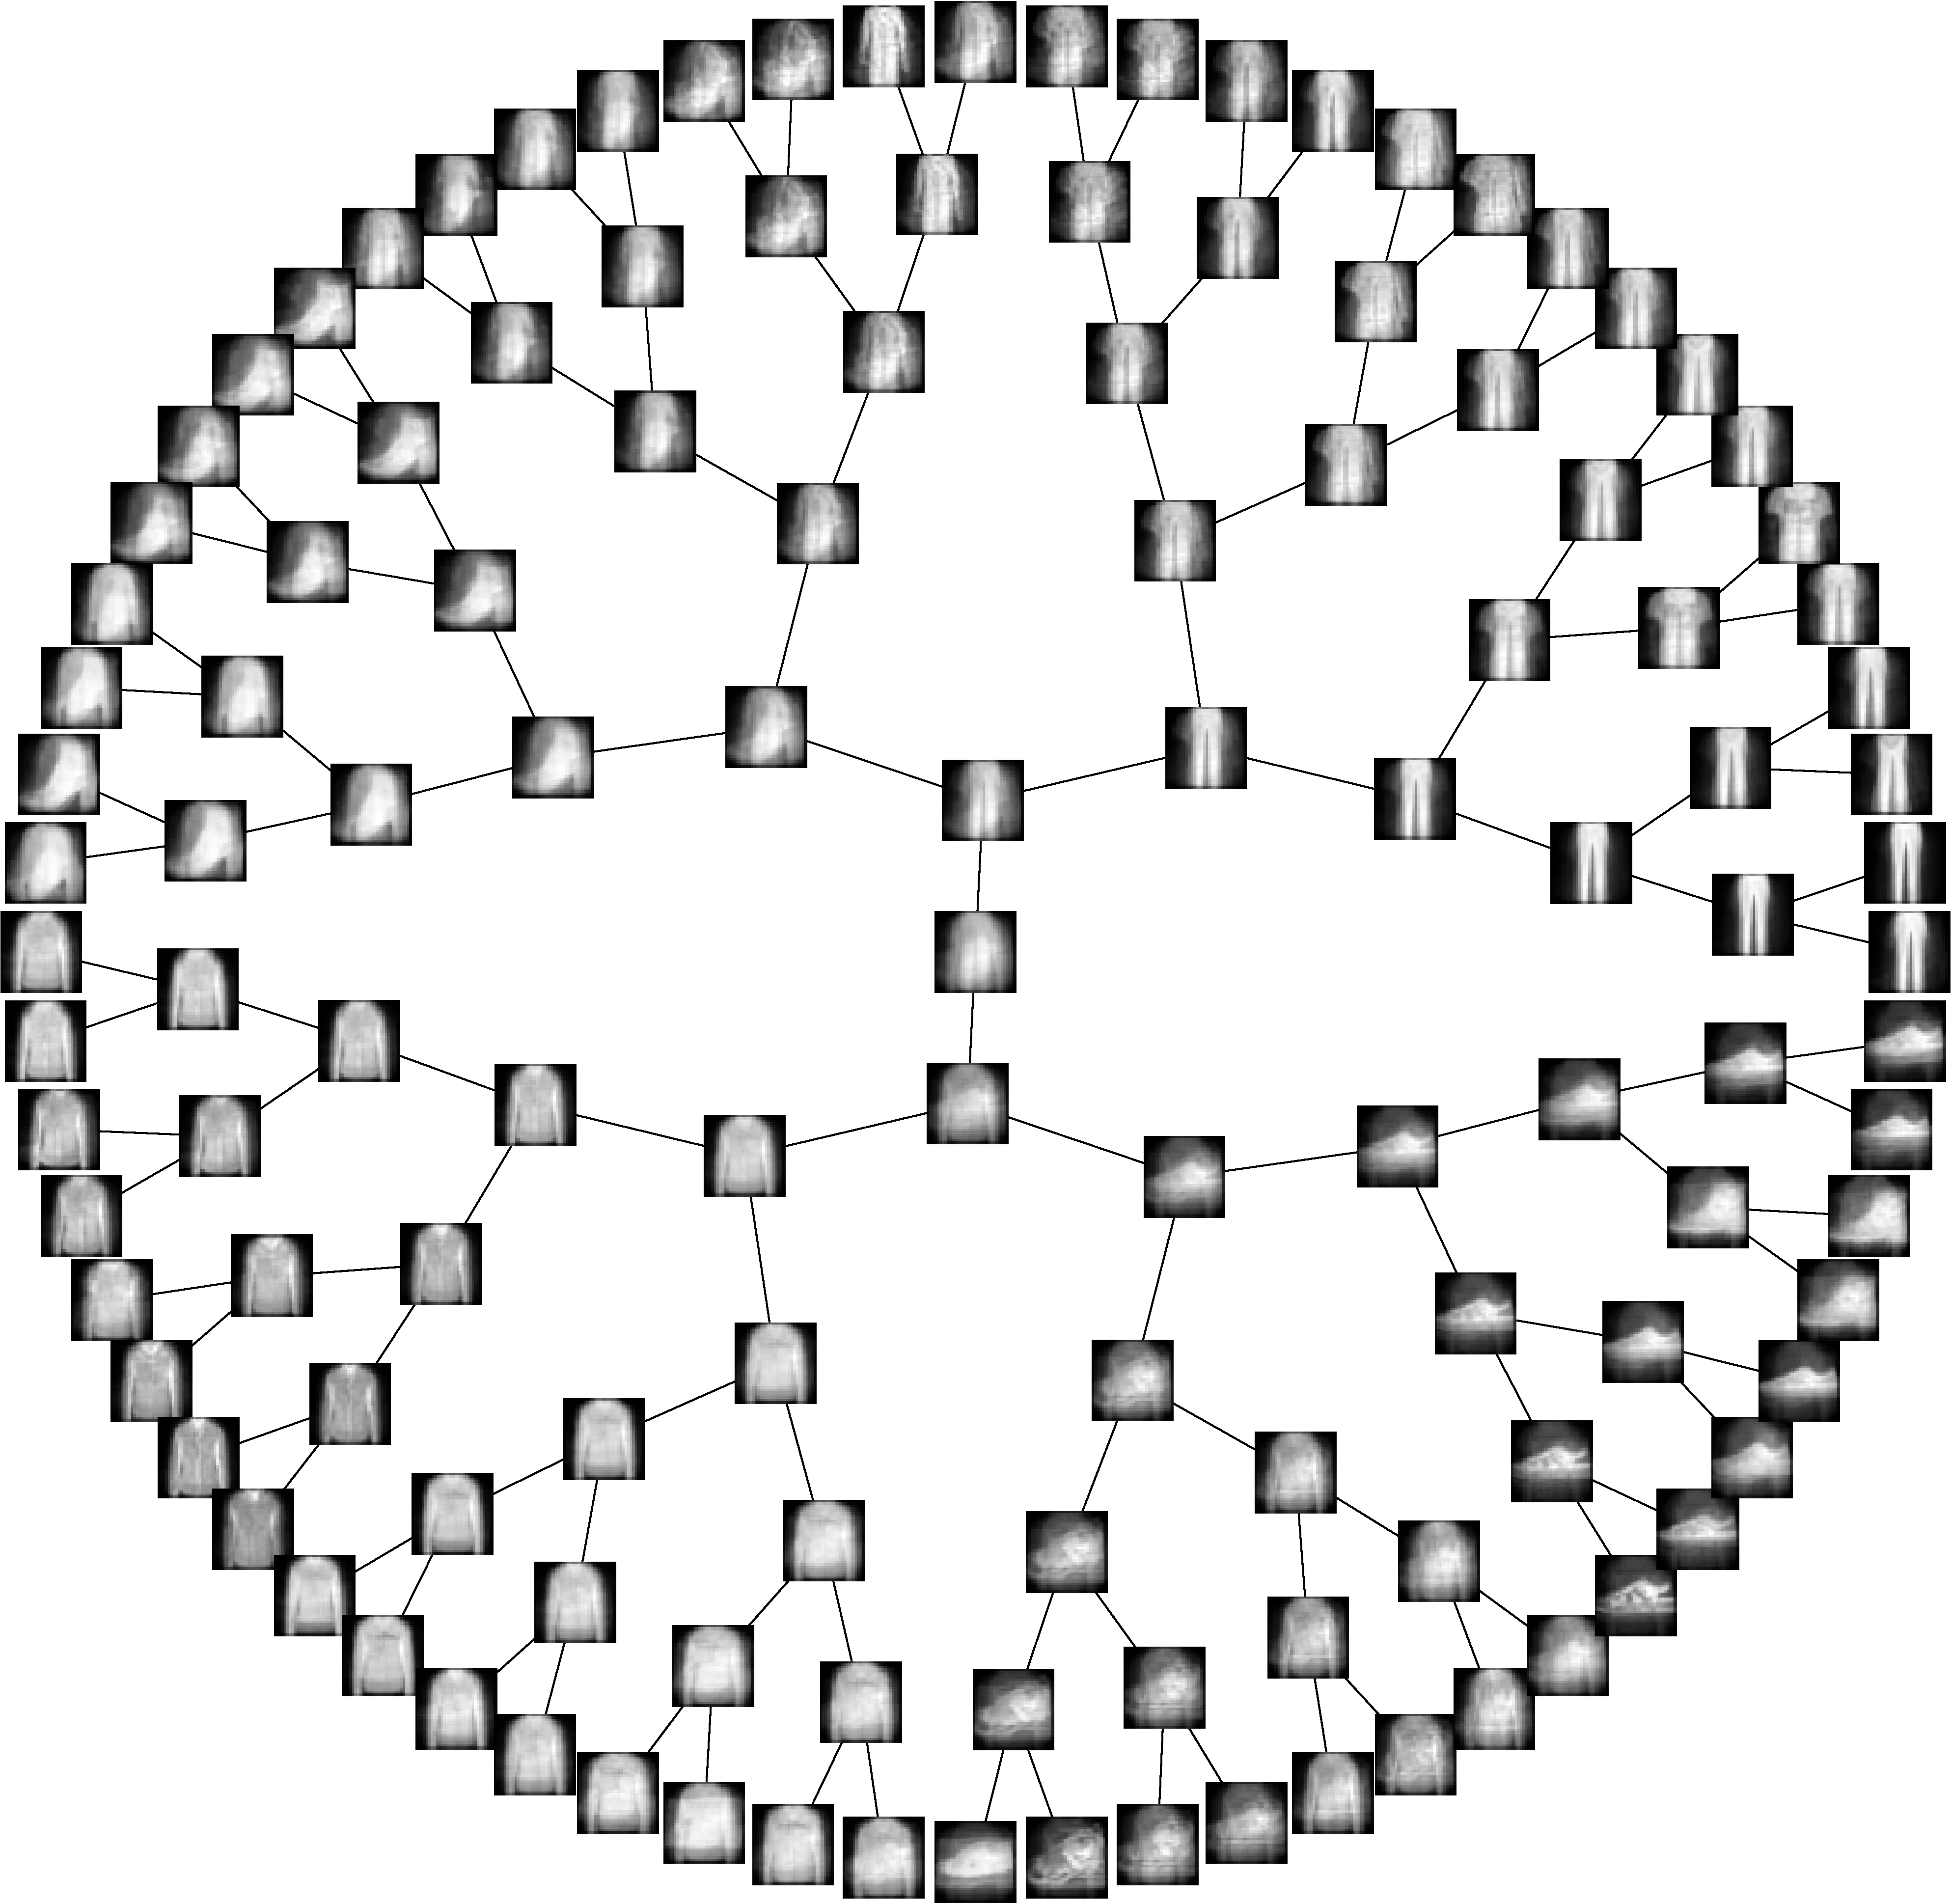
\includegraphics[width=\columnwidth]{polar_fashion.pdf}
\end{center}
\caption{Mean responses of each node. At the center, there is the root. As we go outer, the depth increases and therefore granularity level increases.}
\vskip\baselineskip % Leave a vertical skip below the figure
\label{fig:polar:fashion}
\end{figure}

\begin{figure}[htbp]
\begin{center}
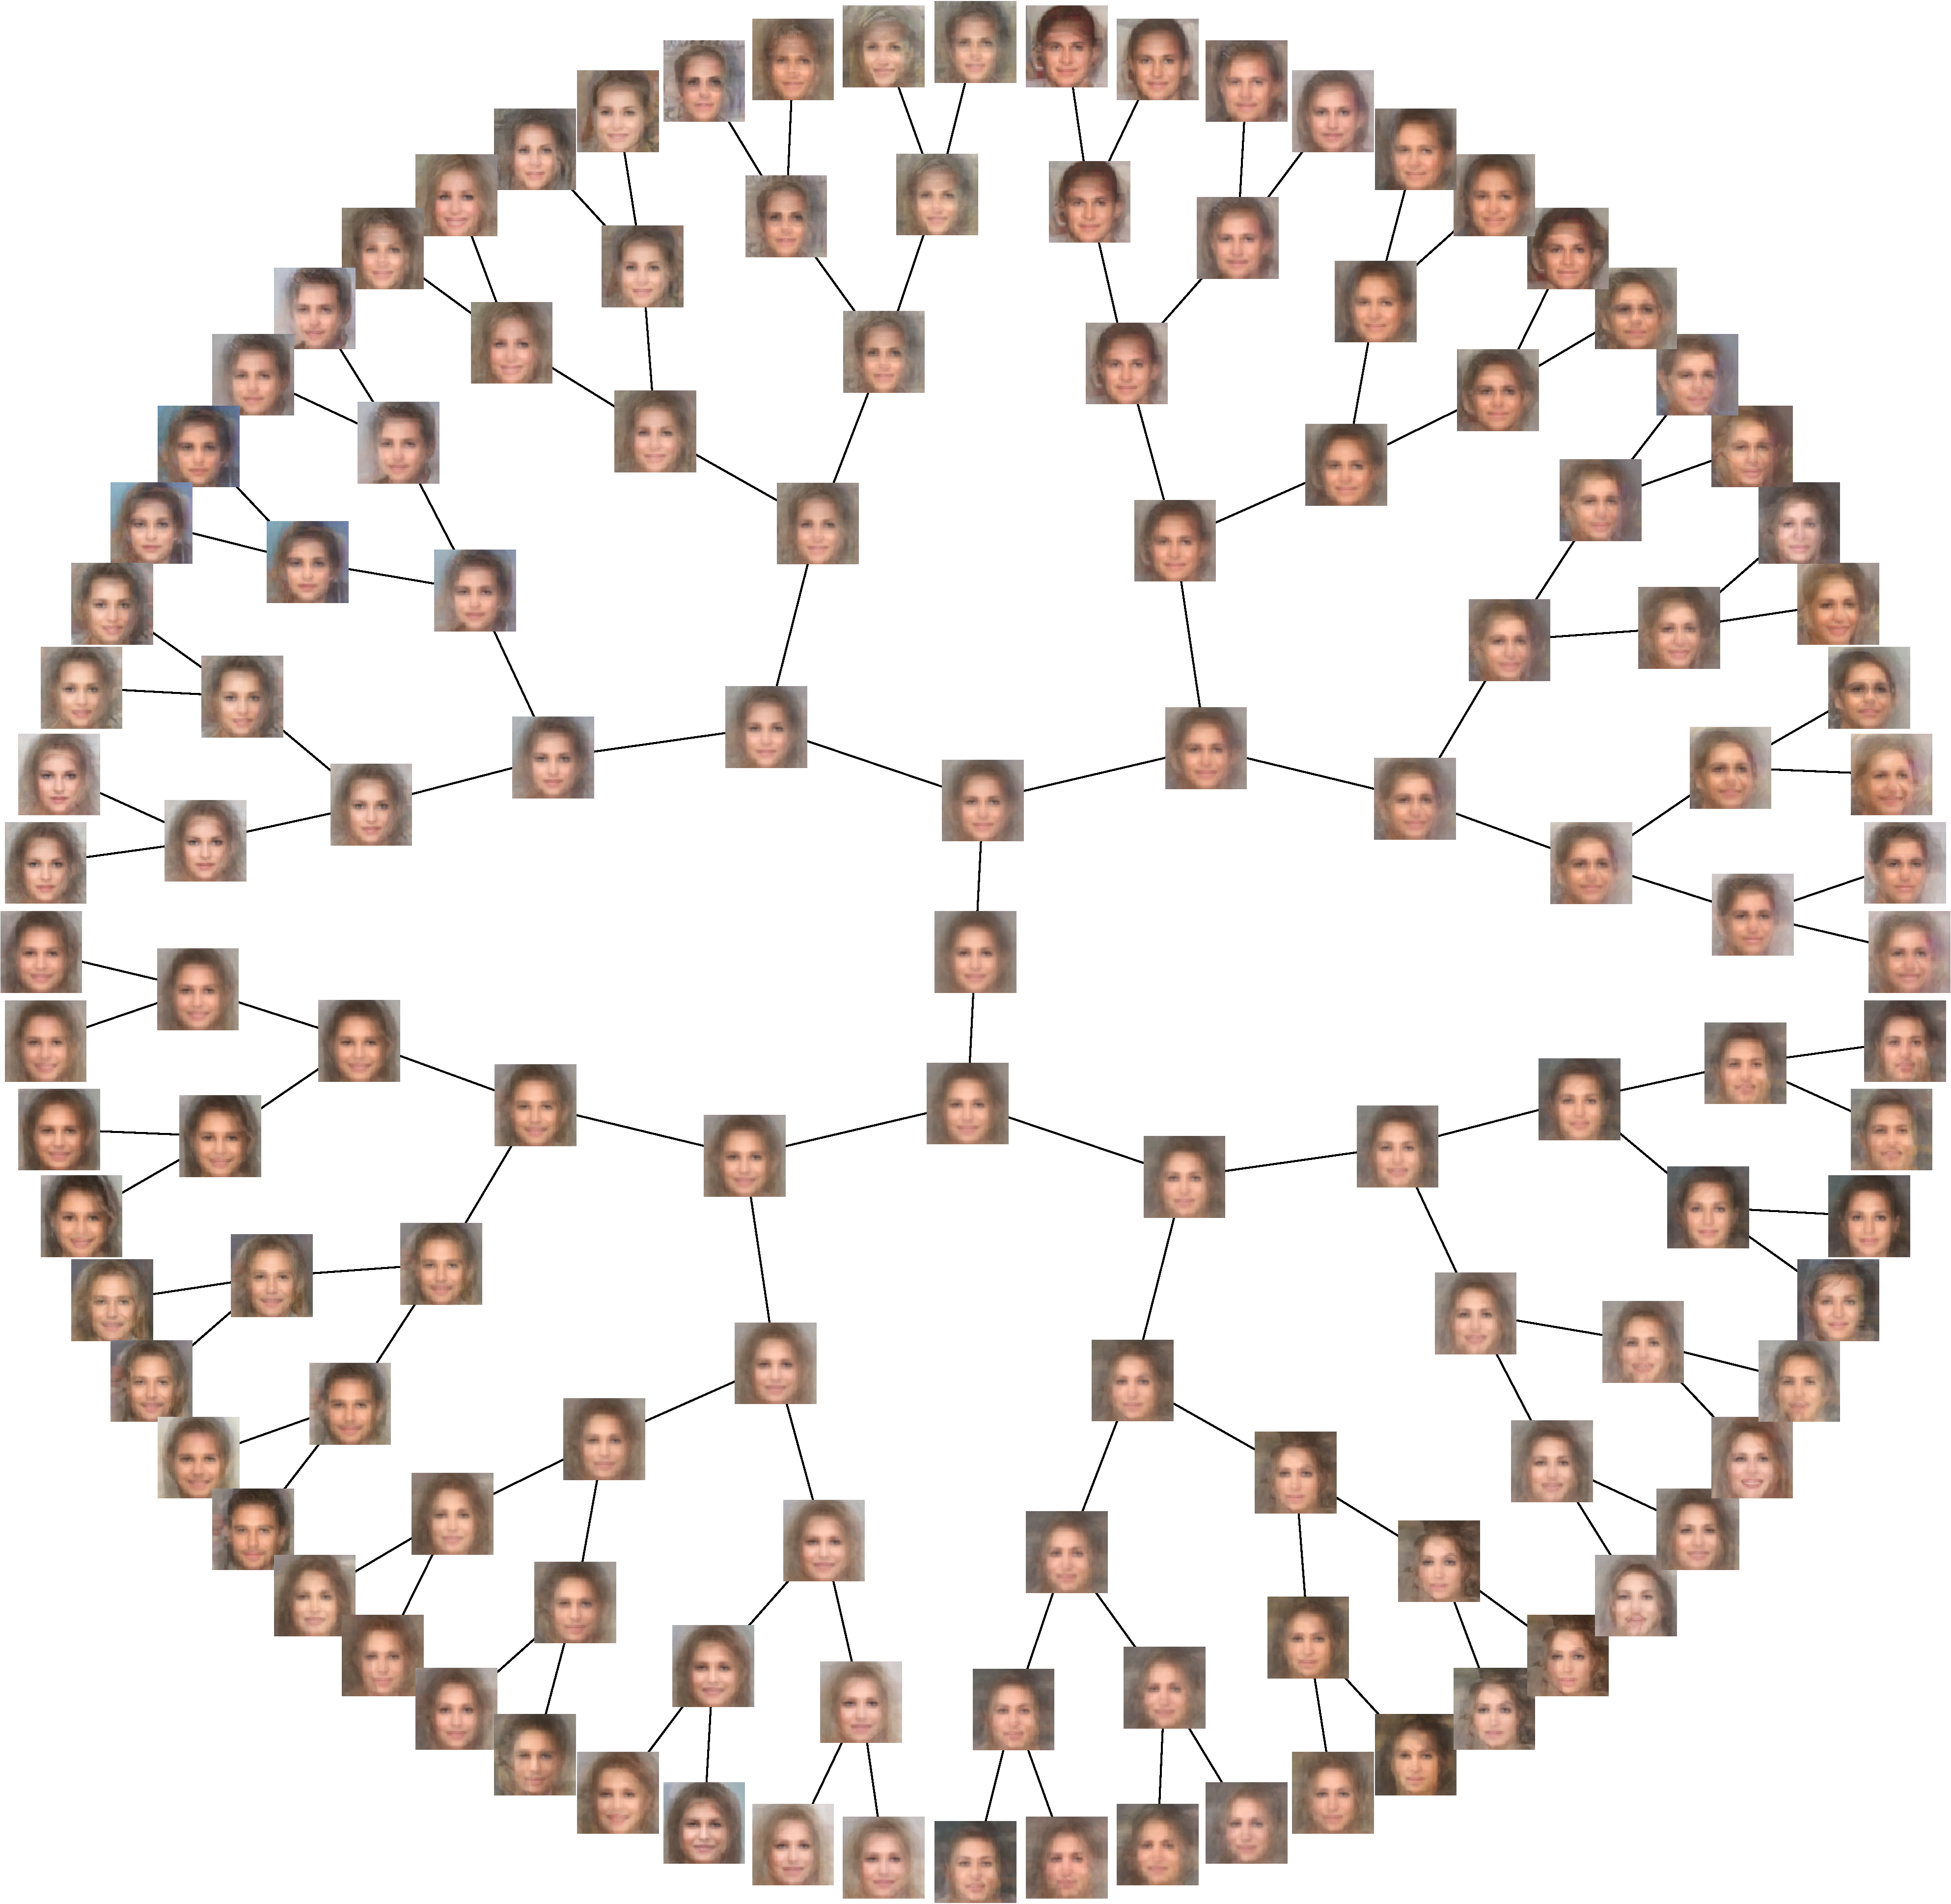
\includegraphics[width=\columnwidth]{polar_celeb.pdf}
\end{center}
\caption{Mean responses of each node. At the center, there is the root. As we go outer, the depth increases and therefore granularity level increases.}
\vskip\baselineskip % Leave a vertical skip below the figure
\label{fig:polar:celeb}
\end{figure}

\begin{figure}[htbp]
\begin{center}
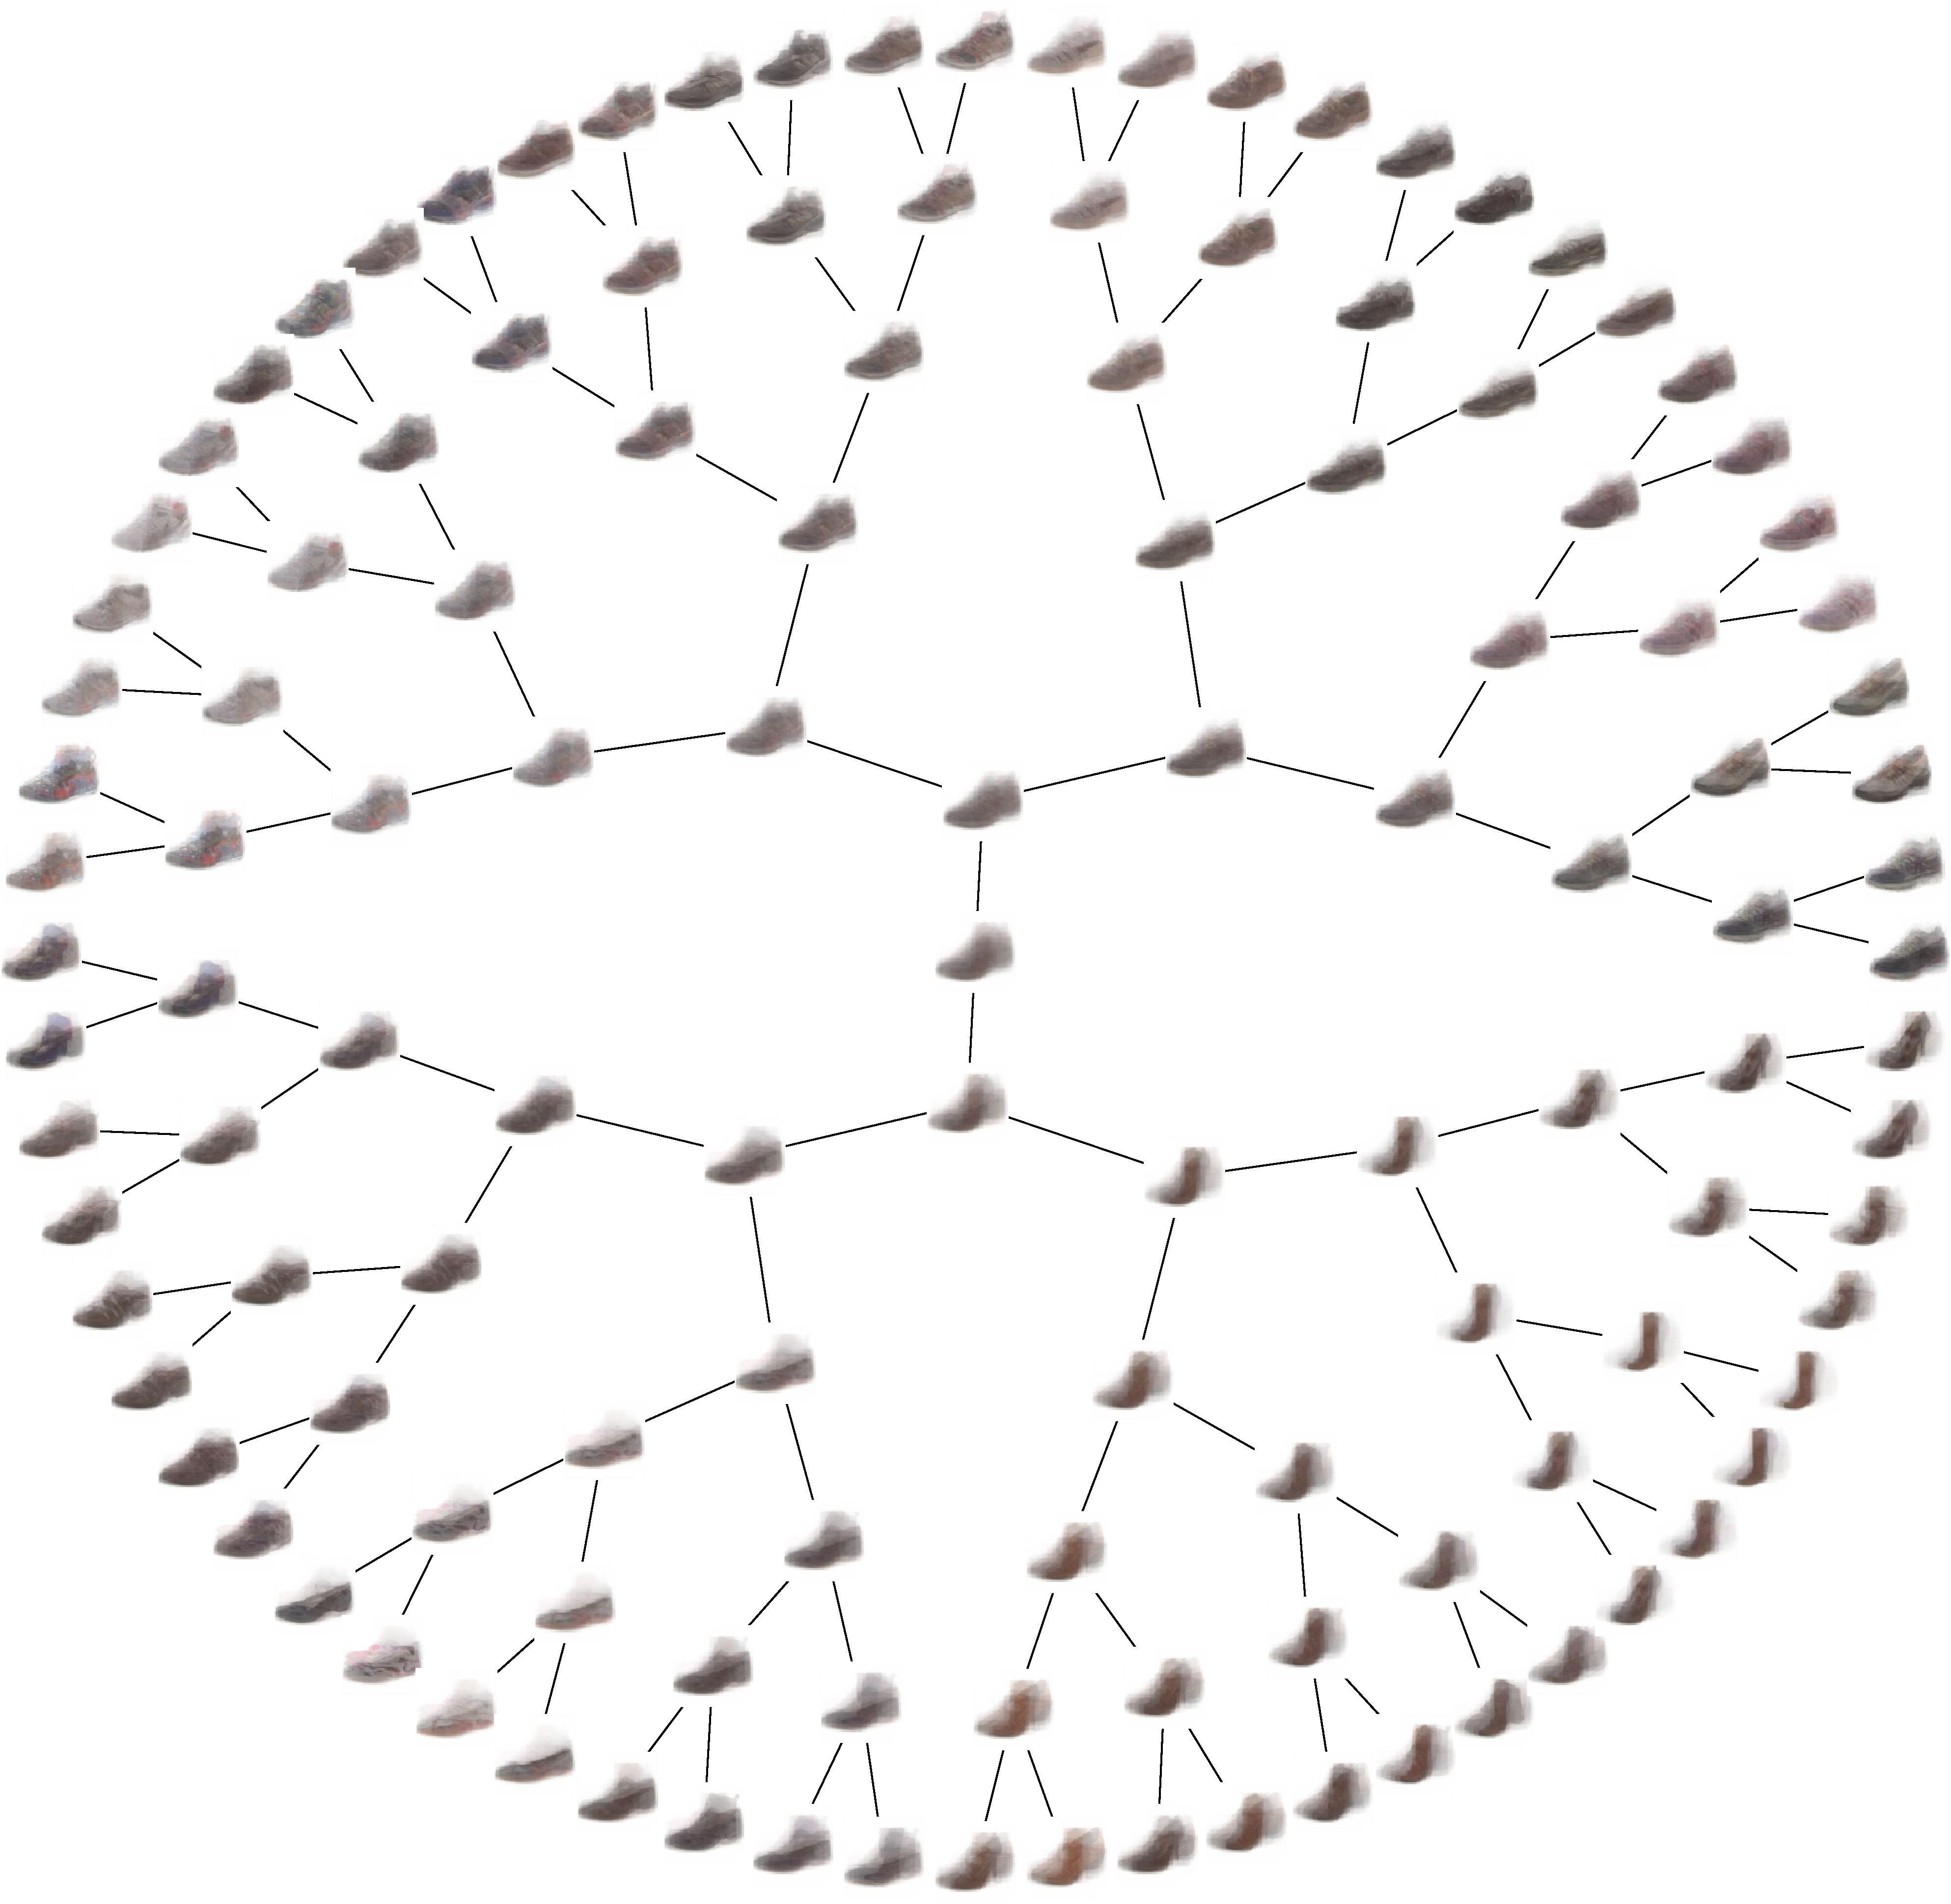
\includegraphics[width=\columnwidth]{polar_utzap50k.pdf}
\end{center}
\caption{Mean responses of each node. At the center, there is the root. As we go outer, the depth increases and therefore granularity level increases.}
\vskip\baselineskip % Leave a vertical skip below the figure
\label{fig:polar:utzap50k}
\end{figure}

\begin{figure}[htbp]
\begin{center}
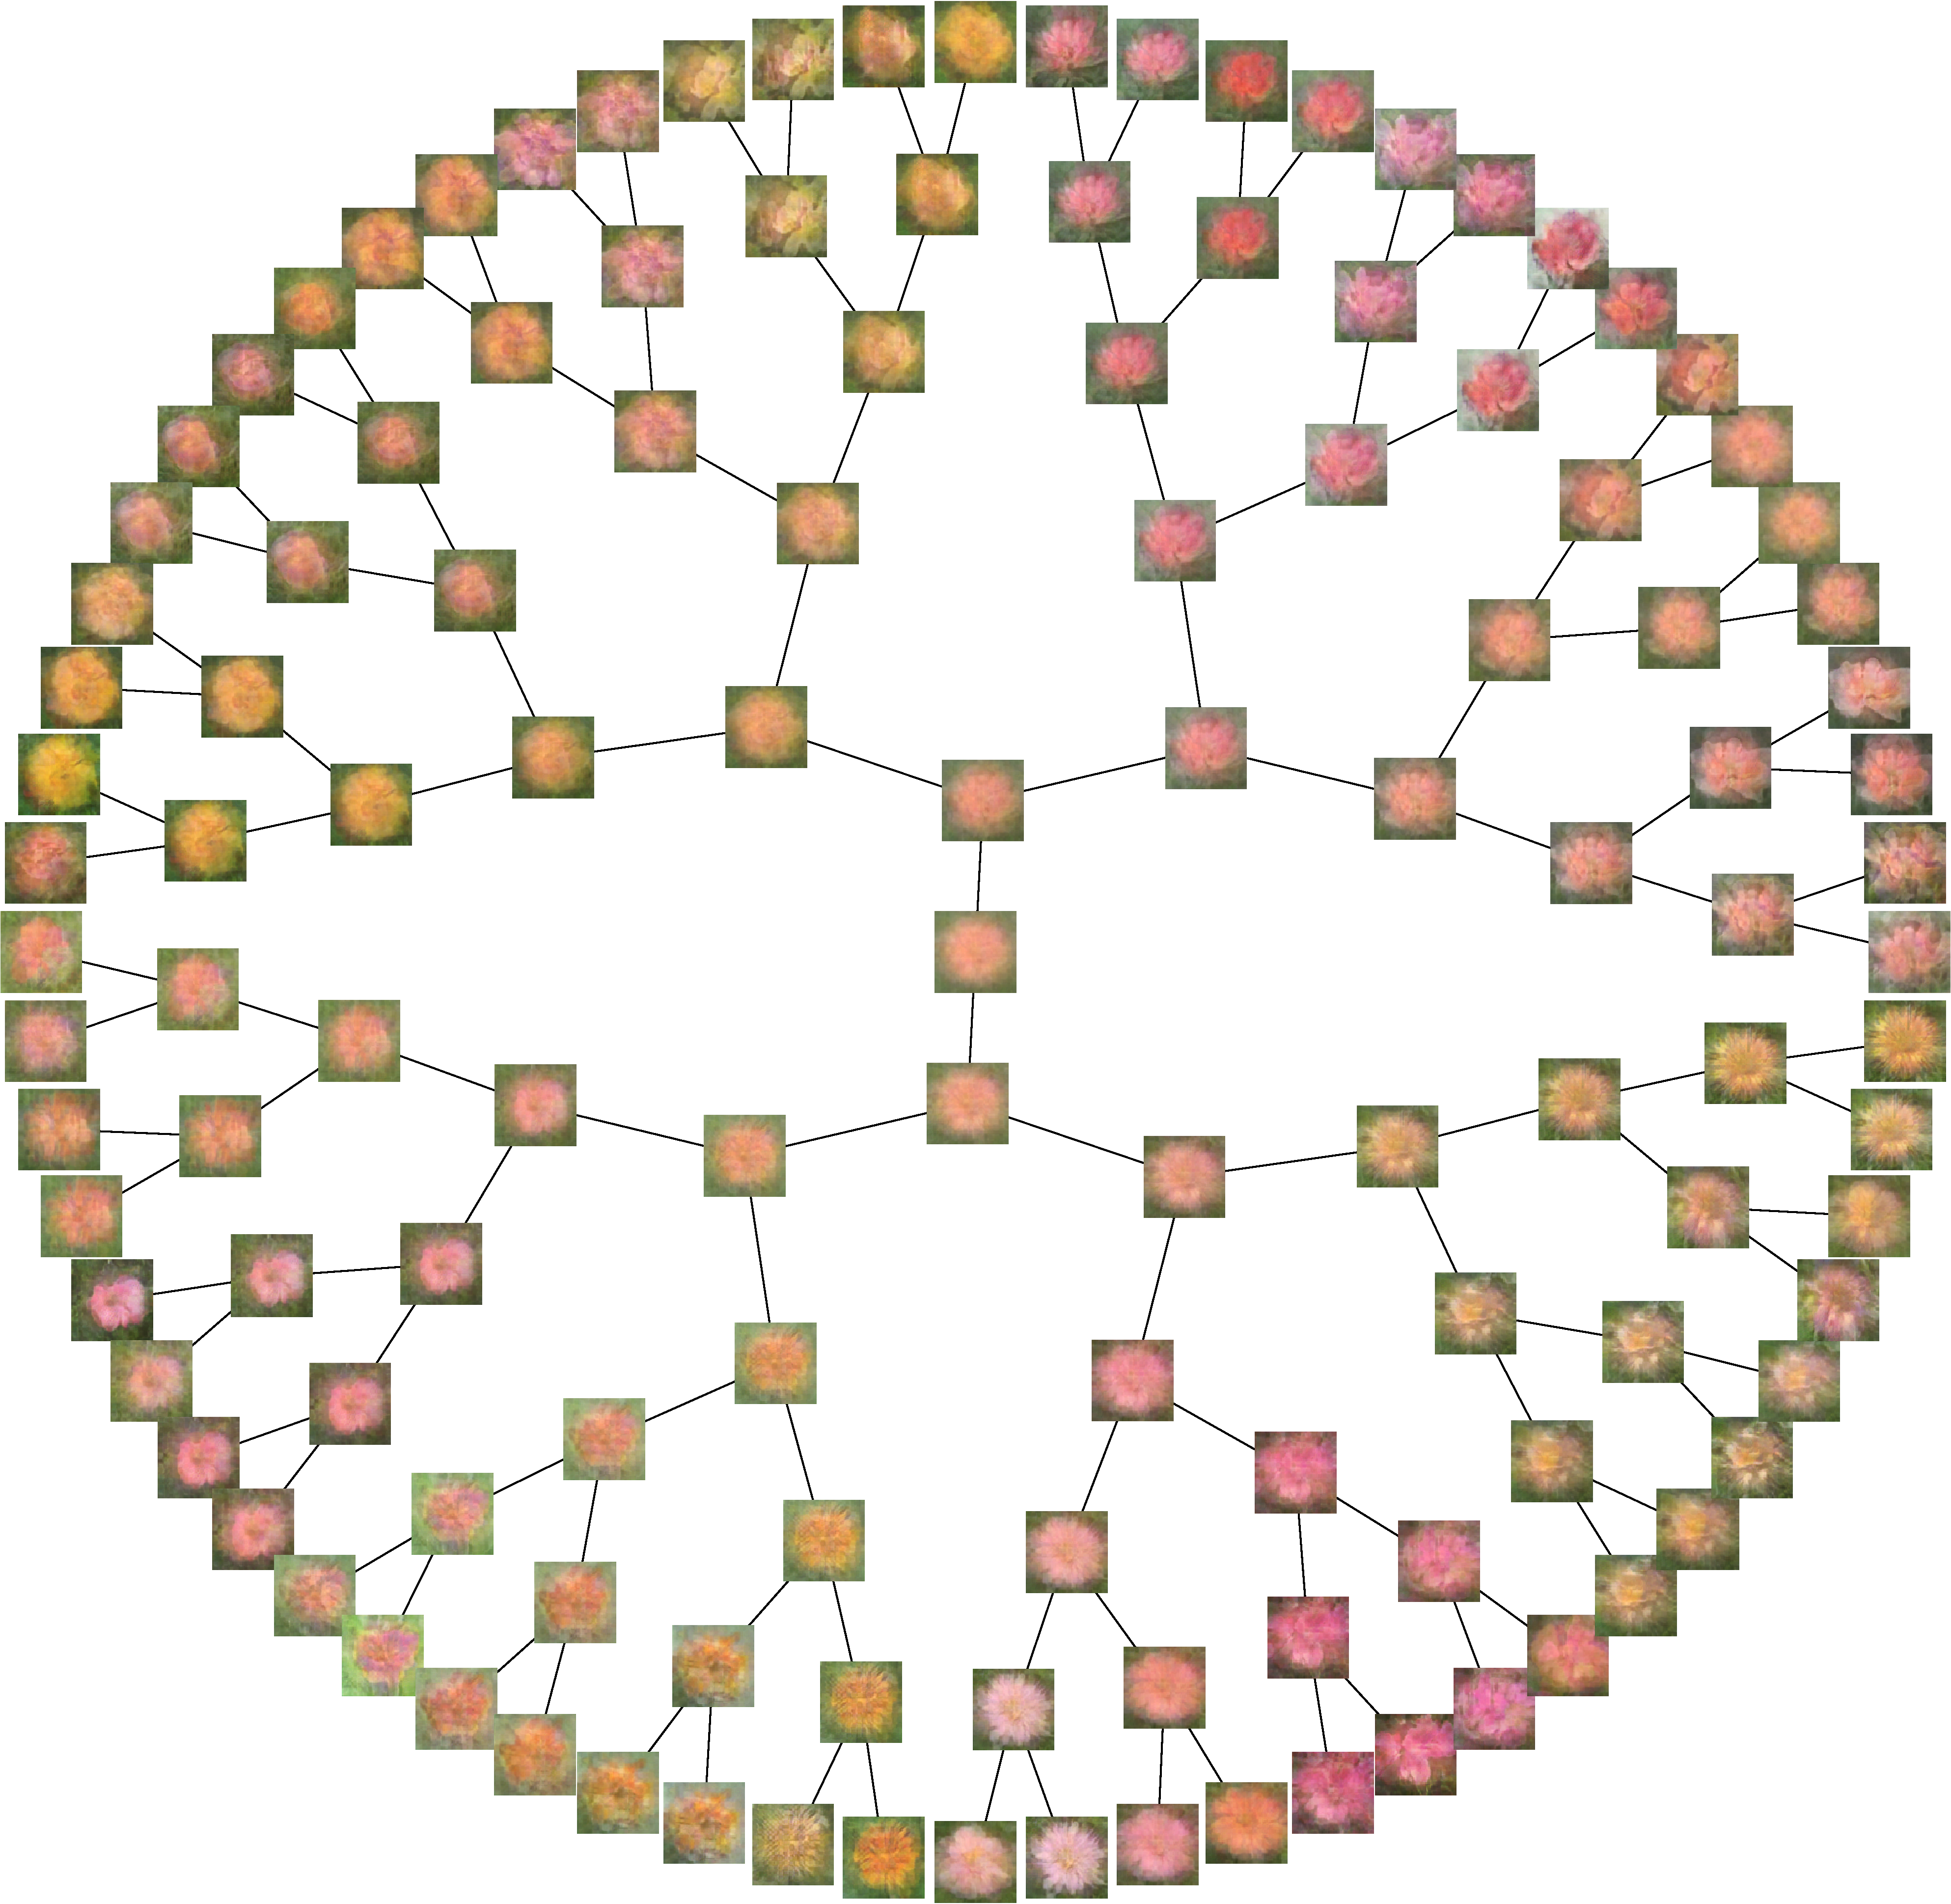
\includegraphics[width=\columnwidth]{polar_flowers.pdf}
\end{center}
\caption{Mean responses of each node. At the center, there is the root. As we go outer, the depth increases and therefore granularity level increases.}
\vskip\baselineskip % Leave a vertical skip below the figure
\label{fig:polar:flowers}
\end{figure}

\begin{figure}[htbp]
\begin{center}
\subfloat[MNIST]{
	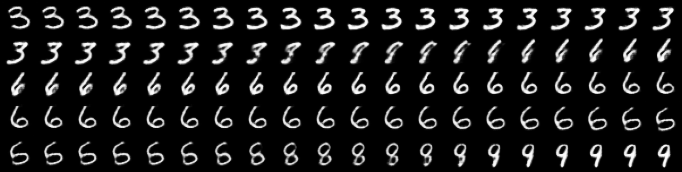
\includegraphics[width=0.8\linewidth]{inter_mnist.png}
	\label{fig:inter:mnist}
}

\subfloat[FashionMNIST]{
	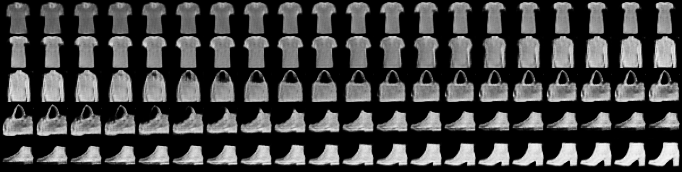
\includegraphics[width=0.8\linewidth]{inter_fashion.png}
	\label{fig:inter:fashion}
}

\subfloat[CelebA]{
	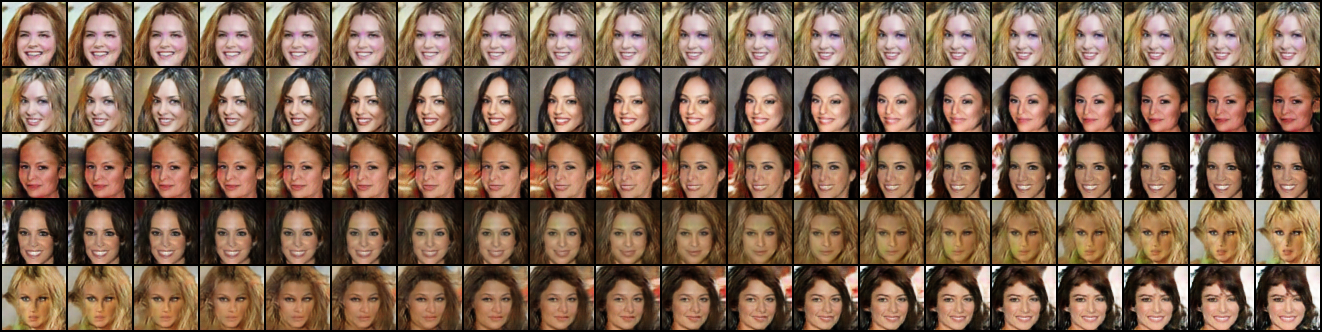
\includegraphics[width=0.8\linewidth]{inter_celeb.png}
	\label{fig:inter:celeb}
}

\subfloat[UTZap50K]{
	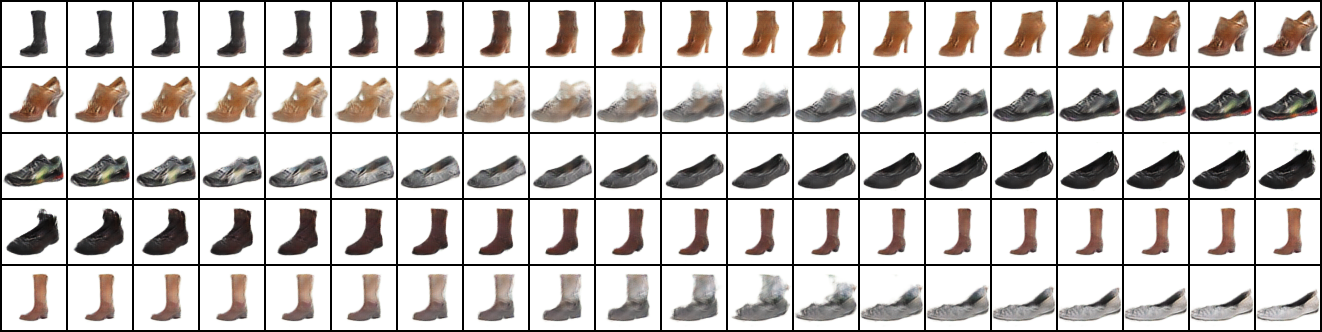
\includegraphics[width=0.8\linewidth]{inter_utzap50k.png}
	\label{fig:inter:utzap50k}
}

\subfloat[Oxford Flowers]{
	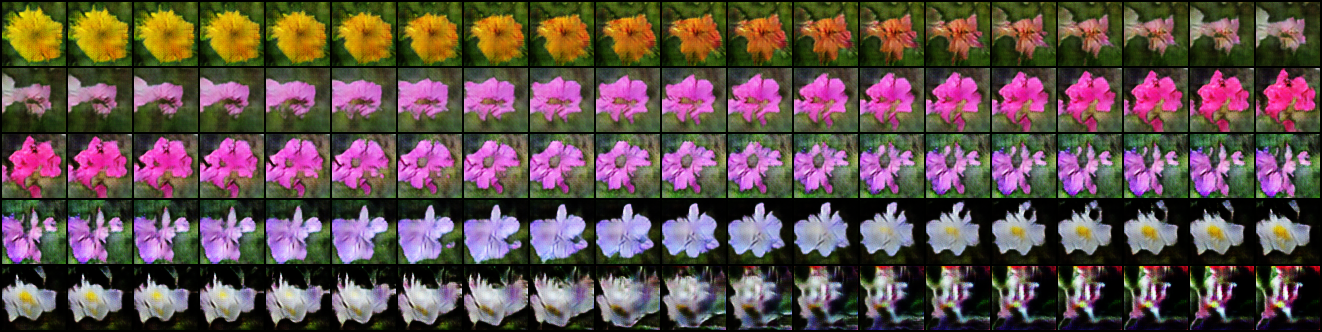
\includegraphics[width=0.8\linewidth]{inter_flowers.png}
	\label{fig:inter:flowers}
}
\end{center}
\caption{Interpolation between random $z$ vectors with HME-6 model.}
\vskip\baselineskip
\label{fig:interpolations}
\end{figure}

\chapter{CONCLUSION}
\label{chapter:conc}
We propose a hierarchical mixture of generators model for GAN. We show that the parameters can be trained using the gradient information. Our experimental results show that the model can generate samples that are realistic and diverse. Though results are not as good as the the fully connected vanilla model, they are promising.

The greatest advantage of the proposed model is interpretability. Since this is a tree architecture, we can make post-hoc analysis to the learned tree to gain insight about the data. The tree structure indicates granularity at different levels and leaves correspond to modes of the distribıtion.

One future direction is to increase complexity at the leaf level; instead of constant leaves as we have now, we can have linear leaves. Another direction is to adapt the tree structure, that is model complexity, as well as parameters, during learning.

\bibliographystyle{styles/fbe_tez_v11}
\bibliography{references}

\end{document}